% interacttfssample.tex
% v1.05 - August 2017

\documentclass[]{interact}\usepackage[]{graphicx}\usepackage[]{xcolor}
% maxwidth is the original width if it is less than linewidth
% otherwise use linewidth (to make sure the graphics do not exceed the margin)
\makeatletter
\def\maxwidth{ %
  \ifdim\Gin@nat@width>\linewidth
    \linewidth
  \else
    \Gin@nat@width
  \fi
}
\makeatother

\definecolor{fgcolor}{rgb}{0.345, 0.345, 0.345}
\newcommand{\hlnum}[1]{\textcolor[rgb]{0.686,0.059,0.569}{#1}}%
\newcommand{\hlstr}[1]{\textcolor[rgb]{0.192,0.494,0.8}{#1}}%
\newcommand{\hlcom}[1]{\textcolor[rgb]{0.678,0.584,0.686}{\textit{#1}}}%
\newcommand{\hlopt}[1]{\textcolor[rgb]{0,0,0}{#1}}%
\newcommand{\hlstd}[1]{\textcolor[rgb]{0.345,0.345,0.345}{#1}}%
\newcommand{\hlkwa}[1]{\textcolor[rgb]{0.161,0.373,0.58}{\textbf{#1}}}%
\newcommand{\hlkwb}[1]{\textcolor[rgb]{0.69,0.353,0.396}{#1}}%
\newcommand{\hlkwc}[1]{\textcolor[rgb]{0.333,0.667,0.333}{#1}}%
\newcommand{\hlkwd}[1]{\textcolor[rgb]{0.737,0.353,0.396}{\textbf{#1}}}%
\let\hlipl\hlkwb

\usepackage{framed}
\makeatletter
\newenvironment{kframe}{%
 \def\at@end@of@kframe{}%
 \ifinner\ifhmode%
  \def\at@end@of@kframe{\end{minipage}}%
  \begin{minipage}{\columnwidth}%
 \fi\fi%
 \def\FrameCommand##1{\hskip\@totalleftmargin \hskip-\fboxsep
 \colorbox{shadecolor}{##1}\hskip-\fboxsep
     % There is no \\@totalrightmargin, so:
     \hskip-\linewidth \hskip-\@totalleftmargin \hskip\columnwidth}%
 \MakeFramed {\advance\hsize-\width
   \@totalleftmargin\z@ \linewidth\hsize
   \@setminipage}}%
 {\par\unskip\endMakeFramed%
 \at@end@of@kframe}
\makeatother

\definecolor{shadecolor}{rgb}{.97, .97, .97}
\definecolor{messagecolor}{rgb}{0, 0, 0}
\definecolor{warningcolor}{rgb}{1, 0, 1}
\definecolor{errorcolor}{rgb}{1, 0, 0}
\newenvironment{knitrout}{}{} % an empty environment to be redefined in TeX

\usepackage{alltt}

% https://tex.stackexchange.com/questions/2441/how-to-add-a-forced-line-break-inside-a-table-cell
\usepackage{makecell}
\usepackage{epstopdf}% To incorporate .eps illustrations using PDFLaTeX, etc.
\usepackage[caption=false]{subfig}% Support for small, `sub' figures and tables
%\usepackage[nolists,tablesfirst]{endfloat}% To `separate' figures and tables from text if required

%\usepackage[doublespacing]{setspace}% To produce a `double spaced' document if required
%\setlength\parindent{24pt}% To increase paragraph indentation when line spacing is doubled
%\setlength\bibindent{2em}% To increase hanging indent in bibliography when line spacing is doubled

%%\usepackage[numbers,sort&compress]{natbib}% Citation support using natbib.sty
\usepackage[authoryear]{natbib} % For author-year citations
%%\bibpunct[, ]{[}{]}{,}{n}{,}{,}% Citation support using natbib.sty
\renewcommand\bibfont{\fontsize{10}{12}\selectfont}% Bibliography support using natbib.sty

\theoremstyle{plain}% Theorem-like structures provided by amsthm.sty
\newtheorem{theorem}{Theorem}[section]
\newtheorem{lemma}[theorem]{Lemma}
\newtheorem{corollary}[theorem]{Corollary}
\newtheorem{proposition}[theorem]{Proposition}

\theoremstyle{definition}
\newtheorem{definition}[theorem]{Definition}
\newtheorem{example}[theorem]{Example}

\theoremstyle{remark}
\newtheorem{remark}{Remark}
\newtheorem{notation}{Notation}

%%%%%%%%%%%%%%
%% CLEVEREF %%
%%%%%%%%%%%%%%
%% order matters: hyperref before cleverref, and biblatex last
\usepackage{hyperref}
% Set up hyperref with desired link colors and border colors
\hypersetup{
  colorlinks=false,          % Disable colored text for links
  %%citebordercolor=0 1 0,     % RGB color for citation link border (green)
  %%citebordercolor=0 0 1,     % RGB color for citation link border (blue)
  %%linkbordercolor=0 0 1,     % RGB color for internal link border (blue)
  citebordercolor=0 1 1,     % RGB color for citation link border (cyan)
  linkbordercolor=0 1 1,     % RGB color for internal link border (cyan)
  urlbordercolor=0 1 1       % RGB color for URL link border (cyan)
}
%%
%% cleveref package for convenient hyper-referencing/citing:
\usepackage[nameinlink,capitalize]{cleveref}
%% The default cref format includes a space before the number, e.g.,
%% "§ 3" rather than "§3", so when using § it looks better to
%% define the cref format explicitly:
%% https://tex.stackexchange.com/questions/247538/remove-space-in-the-default-cref-command
%% \crefformat{section}{\S#2#1#3}
%% A space is still included when multiple sections are referenced,
%% but I think removing the space for multiple section refs would look
%% worse.
%% revised for BMB:
%%\crefname{section}{\S}{\S\S}
\crefname{section}{Sect.}{Sects.}
\Crefname{section}{Section}{Sections}
\crefname{equation}{Eq.}{Eqs.}
\Crefname{equation}{Equation}{Equations}
\crefname{figure}{Fig.}{Figs.}
\Crefname{figure}{Figure}{Figures}
\Crefname{appsec}{Appendix}{appendices}

%% other DE preamable
\usepackage{pdflscape} % landscape mode that rotates page (unlike lscape)
\usepackage{xcolor}
\usepackage{lineno}\renewcommand\thelinenumber{\color{gray}\arabic{linenumber}}
\usepackage{placeins}
\newcommand{\thickredline}{{\color{red}\bigskip\begin{center}\linethickness{2mm}\line(1,0){250}\end{center}\bigskip}}
\newcommand{\bmb}[1]{{\color{red}$\langle$\emph{BMB: #1}$\rangle$}}
\newcommand{\swp}[1]{{\color{blue}$\langle$\emph{SWP: #1}$\rangle$}}
\newcommand{\djde}[1]{{\color{magenta}$\langle$\emph{DJDE: #1}$\rangle$}}
%%\newcommand{\djde}[1]{\relax}
\newcommand{\needref}{{\color{orange}[NEED REF]}}
\newcommand{\term}[1]{{\bfseries\slshape#1}}

%% derivatives
%% note that \d is a built-in accent macro
\newcommand{\dee}{{\rm d}}
\newcommand{\dd}[2]{{\frac{\dee{#1}}{\dee{#2}}}}
\newcommand{\dbyd}[2]{{{\dee{#1}}/{\dee{#2}}}}
\newcommand{\ddx}[1]{\dd{#1}{x}}
\newcommand{\ddt}[1]{\dd{#1}{t}}
\newcommand{\ddtau}[1]{\dd{#1}{\tau}}
\newcommand{\dbydx}[1]{\dbyd{#1}{x}}
\newcommand{\dbydt}[1]{\dbyd{#1}{t}}
\newcommand{\dbydtau}[1]{\dbyd{#1}{\tau}}
\newcommand{\dt}{\dee t}

\newcommand{\sech}{\,\textrm{sech}}
\newcommand{\Ipeak}{I_{\rm p}}
\newcommand{\tpeak}{t_{\rm p}}
\newcommand{\R}{{\mathcal R}}
\newcommand{\Rn}{\R_0}
\newcommand{\Tg}{T_{\rm g}}
\newcommand{\Reff}{\R_{\rm e}}
\usepackage{xspace}
%%\newcommand{\KM}{{KM}\xspace}
%%\newcommand{\KMpage}[1]{\KM [p.\,#1]}
\newcommand{\KM}{\protect\hyperlink{cite.KermMcKe27}{KM}\xspace}
\newcommand{\KMpage}[1]{\protect\hyperlink{cite.KermMcKe27}{KM [p.\,#1]}\xspace}
%% similar style to \citep:
\newcommand{\KMpagep}[1]{[\protect\hyperlink{cite.KermMcKe27}{KM, p.\,#1}]\xspace}
\usepackage{bm} % bold math
\newcommand{\fvec}{{\bm{f}}}
\newcommand{\Phivec}{{\bm{\Phi}}}
\newcommand{\xvec}{{\bm{x}}}
\newcommand{\thetavec}{{\bm{\theta}}}
\newcommand{\thetavechat}{{\bm{\hat\theta}}}
%%\newcommand{\gradtheta}{\nabla_{\!\!\thetavec}}
\newcommand{\gradtheta}{\nabla_{{}_{\!\!\thetavec}}}
%%\newcommand{\gradx}{\nabla_{\!\!\xvec}}
\newcommand{\gradx}{\nabla_{{}_{\!\!\xvec}}}
\newcommand{\code}[1]{\texttt{\detokenize{#1}}}
\usepackage{xspace}
%% modify these based on whether we're using Okabe-Ito or not
\newcommand{\KMcol}{blue\xspace}  %% the same both ways
\newcommand{\nlscol}{orange\xspace}  %% was: red
\newcommand{\FOolscol}{light blue\xspace} % was: grey
\newcommand{\FOnbcol}{gold\xspace}
\newcommand{\determcol}{green\xspace}
\newcommand{\Prob}{{\mathbb{P}}} % probability operator (measure)
%% two ways to get lower case black board bold:
%% this one just allows lower case in \mathbb:
%%\usepackage{bbold} % lower case blackboard bold
%%\newcommand{\pdens}{{\mathbm{p}}} % probability density
%% I like this bb font better, which requires the \mathbbm macro for
%% lower case:
\usepackage{bbm} % lower case blackboard bold
\newcommand{\pdens}{{\mathbbm{p}}} % probability density
\newcommand{\pdenstindex}{\pdens_{{}_{\tindex}}}
%% keep this one around for building diffs
\newcommand{\Pop}{{\mathbbm{P}}} % probability density
\newcommand{\lik}{{\mathcal L}}
\newcommand{\transpose}{{\textsf{T}}}
\DeclareMathOperator*{\argmax}{arg\,max}
\DeclareMathOperator*{\argmin}{arg\,min}
\newcommand{\normdist}{\ensuremath\mathrm{Normal}}
%% tables
\usepackage{multirow}   % for tables
%\usepackage{subfig}
\usepackage{tabularx}   % pretty tables
% \usepackage{tabularray} % allows rowsep via tblr environment
%% table details
\renewcommand{\arraystretch}{1.5} % more interline spacing
%% https://tex.stackexchange.com/questions/12703/how-to-create-fixed-width-table-columns-with-text-raggedright-centered-raggedlef
\usepackage{ragged2e}
%%\usepackage{array} % for m{...}
\newcommand\ttbackslash{{\tt\char`\\}}
\newcommand{\macro}[1]{{\tt\ttbackslash#1}}
\newcommand{\traj}{x}
\newcommand{\ie}{i.e., }
\newcommand{\sens}{{\mathsf S}}
\newcommand{\sensmat}{{\bm{\sens}}}
\newcommand{\tindex}{{\ell}}
\newcommand{\ti}{t_\tindex}
\newcommand{\timo}{t_{\tindex-1}}
\newcommand{\tindexmax}{{n_t}}
\newcommand{\xindex}{{i}}
\newcommand{\xindexmax}{{n_{{}_x}}}
\newcommand{\thetaindex}{{j}}
\newcommand{\thetaindexmax}{{n_{{}_\theta}}}
%% observed values
\newcommand{\trajobssymbol}{\traj_{{\rm{\color{black}\scalebox{0.5}{obs}}}}}
\newcommand{\trajobs}[1]{\trajobssymbol\!\left(#1\right)}
\newcommand{\trajobsti}{\trajobs{\ti}}
%%\newcommand{\trajobsiti}{{\trajobssymbol}_{,\xindex}(\ti)}
\newcommand{\trajobsi}{\traj_{{\rm{\color{black}\scalebox{0.5}{obs}}},\xindex}}
\newcommand{\trajobsiti}{\trajobsi(\ti)}
\newcommand{\xvecobssymbol}{\xvec_{{\rm{\color{black}\scalebox{0.5}{obs}}}}}
\newcommand{\xvecobs}[1]{\xvecobssymbol\!\left(#1\right)}
\newcommand{\xvecobsti}{\xvecobs{\ti}}

%% initial state:
%% \newcommand{\Sinit}{S_{\rm i}}
%% \newcommand{\Iinit}{I_{\rm i}}
%% \newcommand{\Rinit}{R_{\rm i}}
\newcommand{\Sinit}{S(0)}
\newcommand{\Iinit}{I(0)}
\newcommand{\Rinit}{R(0)}



\IfFileExists{upquote.sty}{\usepackage{upquote}}{}
\begin{document}

\articletype{ORIGINAL ARTICLE}% Specify the article type or omit as appropriate
\articletype{Article type: \ EDUCATION}

\title{Fitting epidemic models to data -- a tutorial\\in memory of Fred
  Brauer}

\author{
  \name{David J.\,D.~Earn\textsuperscript{a}\thanks{%%CONTACT
    D.J.D.~Earn. \href{mailto:earn@math.mcmaster.ca}{earn@math.mcmaster.ca}. ORCID: 0000-0002-7562-1341}, %%%Twitter: @David.J.D.Earn},
    Sang Woo Park\textsuperscript{b}\thanks{S.W.~Park. \href{mailto:swp2@princeton.edu}{swp2@princeton.edu}. ORCID 0000-0003-2202-3361,} %%% Mastodon: @sangwoopark@ecoevo.social},
    and Benjamin M.~Bolker\textsuperscript{a,c}\thanks{B.M.~Bolker. \href{mailto:bolkerb@mcmaster.ca}{bolkerb@mcmaster.ca}. ORCID: 0000-0002-2127-0443}, %%%Twitter: @bolkerb, Mastodon: @bbolker@fediscience.org}}
  }
  \affil{\textsuperscript{a}Department of Mathematics and Statistics, McMaster University,\\\ Hamilton, Ontario, Canada, L8S 4K1;\\\medskip
    \textsuperscript{b}Department of Ecology and Evolutionary Biology, Princeton University,\\\ Princeton, NJ 08544;\\\medskip
    \textsuperscript{c}Department of Biology, McMaster University,\\\ Hamilton, Ontario, Canada, L8S 4K1}
}

\maketitle

\linenumbers

\bigskip \bigskip

\begin{abstract}
  Fred Brauer was an eminent mathematician who studied dynamical
  systems, especially differential equations.  He made many
  contributions to mathematical epidemiology, a field that is strongly
  connected to data, but he always chose to avoid data analysis.
  Nevertheless, he recognized that fitting models to data is usually
  necessary when attempting to apply infectious disease transmission
  models to real public health problems.  He was curious to know how
  one goes about fitting dynamical models to data, and why it can be
  hard.  Initially in response to Fred's questions, we developed a
  user-friendly \code{R} package, \code{fitode}, that facilitates
  fitting ordinary differential equations to observed time series.
  Here, we use this package to provide a brief tutorial introduction
  to fitting compartmental epidemic models to a single observed time
  series.  We assume that, like Fred, the reader is familiar with
  dynamical systems from a mathematical perspective, but has limited
  experience with statistical methodology or optimization techniques.
\end{abstract}

\begin{keywords}
  epidemic models; infectious diseases; ordinary differential
  equations; parameter estimation; maximum likelihood; \code{fitode}
\end{keywords}

Submitted to \emph{Bulletin of Mathematical Biology}

\section{Introduction}

In their landmark 1927 paper, \citet[p.\,713]{KermMcKe27} (\KM)
introduced the now-standard susceptible-infected-removed (SIR)
epidemic model,
\begin{linenomath*}
  \begin{subequations}\label{eq:SIR}
    \begin{align}
      \ddt{S} &= -\beta S I \,, \label{eq:SIR;S} \\
      \noalign{\vspace{5pt}}
      \ddt{I} &= \beta S I - \gamma I \,, \label{eq:SIR;I}\\
      \noalign{\vspace{5pt}}
      \ddt{R} &= \gamma I\,, \label{eq:SIR;R}
    \end{align}
  \end{subequations}
\end{linenomath*}
where $S$, $I$ and $R$ represent the numbers of individuals who are
susceptible, infected or removed\footnote{In the words of
  \KMpage{701}, ``removed from the number of those who are sick, by
  recovery or by death''.}, $\beta$ is the transmission rate, and
$\gamma$ is the removal (or recovery) rate.  In that original paper,
\KMpage{714} also fit their model to plague mortality data from an
epidemic in Bombay (now Mumbai) that occurred about 20 years before
their paper was written.

In the century that has elapsed since publication of \KM's initial
paper, the field of mathematical epidemiology has expanded and
matured, and has been the subject of many books
\citep{Bart60,Bail75,AndeMay91,AndeBrit00b,DiekHees00,BrauCast01,Brau+19}
and review articles \citep{Heth00,Earn+02,Earn08,Earn09}.  Researchers
have primarily focused on \term{compartmental models} like the SIR
model, cast either as differential equations following the tradition
of \KM, or as \term{stochastic processes} in the
tradition of \citet{McKe26} and \citet{Bart60}.  In
recent years, as the power of computers has grown, some researchers
have turned to \term{agent-based models}, which represent each
individual as a separate unit that can have unique properties
\citep{eubank2004modelling}.

Throughout the history of the subject, and regardless of the modelling
frameworks they have exploited, mathematical epidemiologists have
frequently attempted to fit---or at least to compare---their models to
observed infectious disease data. Such fits have often been
na\"{\i}ve, with limited consideration of their quality. Over the
years, however, there has been a trend towards greater sophistication
and statistical rigour in parameter estimation for infectious disease
models; books that explain these methods have begun to appear in
recent decades \citep{Bolk08,bjorn2018}.  Careful
consideration of uncertainty is especially important when epidemic
models are used for the development and analysis of policy options for
infectious disease management \citep{elderd2006uncertainty}, a
challenge that began to absorb the attention of many mathematical
epidemiologists as soon as the emergence of SARS-CoV-2 ignited the
COVID-19 pandemic \citep{Broo+21,Hill+21,Nixo+22,howerton2023evaluation}.

While visiting the University of British Columbia in 2014--2015, one
of us (DE) had many conversations with Fred Brauer about epidemic
models and how they can be used in practical applications.  While he
had no desire to analyze data himself, Fred was acutely aware that
fitting to data is essential if one wishes to apply epidemic
models to real public health problems, and he did want to understand
what was involved in doing so.

Fred's curiosity inspired us to develop user-friendly software for
fitting ordinary differential equation (ODE) models to observed time
series, with the goal of illustrating the process and challenges of
model fitting to Fred and others like him, i.e., individuals who are
comfortable with mathematical analysis of ODEs but have little or no
experience with statistics and parameter estimation.  Unfortunately,
we have lost the opportunity to present our work to Fred, but it seems
fitting (!) to highlight Fred's role in the history of this work, and
to dedicate this tutorial to his memory.\footnote{We had originally
intended to submit this paper to a collection in honour of Fred's memory
\citep{Kribvand23}.}

\section{Kermack and McKendrick's fit}

We begin by revisiting \KM's
application of their SIR model \eqref{eq:SIR} to the epidemic of
plague in Bombay in 1905--1906.  The observed data (dots in
\cref{fig:Bombay}) were weekly numbers of deaths from plague.

Referring to their version of \cref{fig:Bombay}, \KMpage{714} argued
that ``As at least 80 to 90 per cent.\ of the cases reported terminate
fatally, the ordinate may be taken as approximately representing
[$\dbydt{R}$] as a function of $t$.''  Since (non-human) computers did
not yet exist \citep{Camp09}, and an exact analytical form for this
function could not be found, they proceeded to assume
\KMpagep{713} that $\frac{\beta}{\gamma}R(t)\ll1$, which
yields the approximate analytical form,
\begin{linenomath*}
\begin{equation}\label{eq:sech}
\ddt{R} \approx a \sech^2{(\omega\,t - \phi)}\,.
\end{equation}
\end{linenomath*}
Noting that the \term{basic reproduction number} is\footnote{$\Rn$ is
the expected number of secondary cases resulting from a primary case
in a wholly susceptible population \citep{AndeMay91}.}
\begin{linenomath*}
\begin{equation}\label{eq:R0def}
\Rn = \frac{N\beta}{\gamma} \,,
\end{equation}
\end{linenomath*}
where $N$ is the total population size,
the assumption that yields \KM's approximation \eqref{eq:sech}
can be written
\begin{linenomath*}
\begin{equation}\label{eq:KMassumption}
\frac{R(t)-\Rinit}{N} \ll \frac{1}{\Rn} \,,
\end{equation}
\end{linenomath*}
(\KM assumed $\Rinit=0$); thus,
\cref{eq:sech} is a good approximation as long as
the proportion of the population that has been infected and
removed since the initial time is much less than $1/\Rn$.

Given \cref{eq:R0def}, the \term{effective reproduction number} at
time $t=0$ is
\begin{linenomath*}
\begin{equation}\label{eq:Reffdef}
\Reff = \frac{\Sinit\beta}{\gamma} \,.
\end{equation}
\end{linenomath*}
In terms of $\Reff$, $\gamma$, $\Sinit$ and $\Iinit$, the parameters
in \cref{eq:sech} can be written\footnote{There is a typographical
  error in equation (31) of \KM: their factor
  $\sqrt{-q}$ should be $(-q)$ in their equivalent of the parameter we
  call $a$.  \citet[\S3]{bacaermodel2012} corrected this error without
  comment.}
\begin{linenomath*}
\begin{subequations}\label{eq:sechparams}
\begin{align}
  \omega &= \frac{\gamma}{2} \sqrt{(\Reff-1)^2 +
           \frac{2\Iinit}{\Sinit}\Reff^2}\,, \label{eq:omega} \\
  \phi &= \textrm{arctanh}\left(\frac{\Reff - 1}{2\,\omega/\gamma}
         \right)\,, \label{eq:phi} \\
  \text{and}\qquad
  a &= \frac{2\,\omega^2 \Sinit}{\gamma\,\Reff^2} \label{eq:a} \,.
\end{align}
\end{subequations}
\end{linenomath*}
The values of these parameters that \KM estimated for the Bombay
plague epidemic are listed in the KM column of \cref{tab:Bombay}.
Using these values, \KM plotted their ``calculated'' curve, which we
have reproduced in \KMcol in \cref{fig:Bombay}.



\section{How to fit the model to the data}

The \KMcol curve in \cref{fig:Bombay} does appear to provide a
reasonable fit to the data, but \KM gave no
indication of how their parameter estimates were obtained.
Whatever their process, they must have engaged in some
sort of \term{trajectory matching}, i.e., adjusting parameter values
until the model---\cref{eq:sech} in their case---is, by some
measure, close to the observed data points.  The most obvious metric
for this purpose is the Euclidean distance between the model curve and
the data.  Thus, a natural \term{objective function} to
minimize is
\begin{linenomath*}
\begin{equation}\label{eq:leastsquares}
\sum_{\tindex=1}^{\tindexmax} \big(\traj(\ti;\thetavec) - \trajobsti\big)^2 \,,
\end{equation}
\end{linenomath*}
where the observed data are the points
$\{(\ti,\trajobsti):\tindex=1,\ldots,\tindexmax\}$, $\thetavec$ is the
vector of parameters, and $\traj(t;\thetavec)$ is the model; for \KM's
problem, the parameter vector is $\thetavec=(a,\omega,\phi)$ and the
model is given by \cref{eq:sech}.  (Note that we write $\trajobs{\cdot}$
when referring to observations of the variable $\traj$ and
$\traj(\cdot\,;\cdot)$ when referring to the model.)
Choosing this objective function is equivalent to assuming that the $\trajobsti$ values are direct (but noisy) observations of the state variable $\traj(t)$. When the connection between the dynamical system and our observations is more complicated, we need to define an explicit \term{observation process}; see \cref{sec:Uncertainty}.
Minimizing
\eqref{eq:leastsquares} with respect to $\thetavec$ would have
required some heroic arithmetic with a pencil and paper in 1927, but
it is a simple task with the aid of a modern computer.

In the following segment of R code, we fit equation \eqref{eq:sech} to
the Bombay plague data (which are included in the \code{fitode}
package that we describe below, as a data frame with columns
\code{week} and \code{mort}).  We exploit R's nonlinear least squares
function (\code{nls}), which attempts to minimize the distance
\eqref{eq:leastsquares} to the data, starting from an initial guess
(\code{start}).

\begin{knitrout}
\definecolor{shadecolor}{rgb}{0.969, 0.969, 0.969}\color{fgcolor}\begin{kframe}
\begin{alltt}
\hlstd{sech} \hlkwb{<-} \hlkwa{function}\hlstd{(}\hlkwc{x}\hlstd{) \{}\hlnum{1}\hlopt{/}\hlkwd{cosh}\hlstd{(x)\}}
\hlstd{KM_approx} \hlkwb{<-} \hlkwa{function}\hlstd{(}\hlkwc{t}\hlstd{,} \hlkwc{a}\hlstd{,} \hlkwc{omega}\hlstd{,} \hlkwc{phi}\hlstd{) \{a} \hlopt{*} \hlkwd{sech}\hlstd{(omega}\hlopt{*}\hlstd{t} \hlopt{-} \hlstd{phi)}\hlopt{^}\hlnum{2}\hlstd{\}}
\hlstd{KM.parameters} \hlkwb{<-} \hlkwd{c}\hlstd{(}\hlkwc{a} \hlstd{=} \hlnum{890}\hlstd{,} \hlkwc{omega} \hlstd{=} \hlnum{0.2}\hlstd{,} \hlkwc{phi} \hlstd{=} \hlnum{3.4}\hlstd{)}
\hlstd{nlsfit} \hlkwb{<-} \hlkwd{nls}\hlstd{(mort} \hlopt{~} \hlkwd{KM_approx}\hlstd{(week, a, omega, phi),}
              \hlkwc{data} \hlstd{= fitode}\hlopt{::}\hlstd{bombay,}
              \hlkwc{start} \hlstd{= KM.parameters)}
\hlstd{nls.parameters} \hlkwb{<-} \hlkwd{coef}\hlstd{(nlsfit)}
\hlkwd{print}\hlstd{(nls.parameters)}
\end{alltt}
\begin{verbatim}
##           a       omega         phi 
## 874.7545749   0.1935916   3.3720557
\end{verbatim}
\end{kframe}
\end{knitrout}

\noindent
Above, we chose as our starting value the fitted parameter values of
\KM.  Our least squares parameter values differ from \KM's by a few
percent (see \cref{tab:Bombay}).  The least squares fitted
function is shown in \nlscol in \cref{fig:Bombay}.

Starting from someone else's fit is not a great way to test the
method, but fortunately the least squares fit for this problem is not
very sensitive to the starting value.
To pick reasonable starting values, it often helps to think about the
meaning of parameters.  For example, in the case of \cref{eq:sech}, it
is useful to note that $a$ is the maximum of the function, and if
write $\omega t - \phi$ as $\omega(t-\tpeak)$ then
\begin{linenomath*}
  \begin{equation}\label{eq:tpeak}
    \tpeak = \frac{\phi}{\omega}
  \end{equation}
\end{linenomath*}
is the \term{peak time} (at which the maximum occurs); both $a$ and
$\tpeak$ can be approximated by looking at the plotted data.  Assuming
$\Iinit/\Sinit\ll1$, $\omega$ is half the initial exponential growth
rate\footnote{From \cref{eq:SIR;I}, the initial exponential growth
rate is $\beta \Sinit - \gamma = \gamma(\Reff-1)$.}, so it can be
approximated easily by plotting the data on a log scale, estimating
the initial slope, and dividing by 2.  Very rough guesses for $a$,
$\tpeak$ and $\omega$ are sufficient to converge on the same fit:

\begin{knitrout}
\definecolor{shadecolor}{rgb}{0.969, 0.969, 0.969}\color{fgcolor}\begin{kframe}
\begin{alltt}
\hlstd{a.guess} \hlkwb{<-} \hlnum{1000}    \hlcom{# crude "by eye" estimate of peak value,}
\hlstd{tpeak.guess} \hlkwb{<-} \hlnum{15}  \hlcom{# peak time,}
\hlstd{omega.guess} \hlkwb{<-} \hlnum{1}   \hlcom{# and half the initial growth rate}
\hlstd{phi.guess} \hlkwb{<-} \hlstd{omega.guess} \hlopt{*} \hlstd{tpeak.guess}
\hlstd{nlsfit} \hlkwb{<-} \hlkwd{nls}\hlstd{(mort} \hlopt{~} \hlkwd{KM_approx}\hlstd{(week, a, omega, phi),}
              \hlkwc{data} \hlstd{= fitode}\hlopt{::}\hlstd{bombay,}
              \hlkwc{start} \hlstd{=} \hlkwd{c}\hlstd{(}\hlkwc{a} \hlstd{= a.guess,} \hlkwc{omega} \hlstd{= omega.guess,}
                        \hlkwc{phi} \hlstd{= phi.guess))}
\hlkwd{print}\hlstd{(nls.parameters} \hlkwb{<-} \hlkwd{coef}\hlstd{(nlsfit))}
\end{alltt}
\begin{verbatim}
##           a       omega         phi 
## 874.7550490   0.1935918   3.3720589
\end{verbatim}
\end{kframe}
\end{knitrout}

\noindent
However, if you experiment with starting values, you will find that if
you pick sufficiently \emph{bad} starting values, then \code{nls} will
fail.  For example, starting from $a=2000$, $\tpeak=5$, and
$\omega=0.1$ yields a ``singular gradient'' error.  More
interestingly, starting from $a=500$, $\tpeak=5$, and $\omega=0.1$
yields $a=869$, $\omega=-0.19$, $\phi=-3.48$, which is far from our
fitted values and illustrates an important fact: there is not
necessarily a unique best fit set of parameters!  In this case, the
alternative solution exists because $\sech^2(x)$ is symmetric about
the $y$ axis, but in general, there can be multiple local minima that
cause nonlinear optimizers to converge to points that may or may not
represent equally good fits to the data.  The potential existence of
multiple local optima makes fitting to data hard; you need to be
cautious, and use common sense, in interpreting the solutions found by
your software (always plot the solutions!). \citet{raue2013lessons}
give suggestions for how to diagnose and handle multiple optima.

If you know that your parameters should be in a certain range, then
you can exclude values outside that range.  For example, to ensure
that all the parameters are non-negative (and exclude the alternative
fit above), you would add the \code{nls} option

\begin{knitrout}
\definecolor{shadecolor}{rgb}{0.969, 0.969, 0.969}\color{fgcolor}\begin{kframe}
\begin{alltt}
\hlstd{lower} \hlkwb{=} \hlkwd{c}\hlstd{(}\hlkwc{a} \hlstd{=} \hlnum{0}\hlstd{,} \hlkwc{omega} \hlstd{=} \hlnum{0}\hlstd{,} \hlkwc{phi} \hlstd{=} \hlnum{0}\hlstd{)}
\end{alltt}
\end{kframe}
\end{knitrout}

\noindent
which would prevent convergence to negative $\omega$ and $\phi$.
Alternatively, you could write
\begin{linenomath*}
  \begin{equation}\label{eq:loglink}
    a=e^A,\quad \omega=e^\Omega,\quad \phi=e^\Phi \,,
  \end{equation}
\end{linenomath*}
and fit $A$, $\Omega$, and $\Phi$, which would guarantee positive $a$,
$\omega$, and $\phi$ without having to constrain the values of the
fitted parameters.  While this last suggestion may just seem like a
cute trick, there is more to it than that.  Many more optimization
algorithms are available for unconstrained fitting; numerical
parameter values of very small magnitude can also lead to numerical
instability, so it is advantageous to link parameters that must lie in
a given range to unconstrained parameters that can be fit more easily
\citep[pp.\,328--329]{Bolk08}.  In \cref{eq:loglink}, the \term{link
  function} that converts the parameters to the unconstrained scale is
$\log(x)$.  Another common link function is
$\textrm{logit}(x) = \log(x/(1-x))$ (the log-odds function, or the
inverse of the logistic function), which converts the unit interval
$(0,1)$ to $(-\infty,\infty)$, and is convenient when parameters
represent proportions or probabilities.  (Requiring positivity is so
common that \code{fitode} uses a log link for all parameters by
default.)





If we accept our fit as satisfactory, what can we infer about the
dynamics of plague that \KM were attempting to capture with the SIR
model \eqref{eq:SIR}?  We need to convert the parameters of \KM's
approximation \eqref{eq:sechparams} back to the original parameters
that are directly related to the mechanism of disease spread formalized by the model (i.e., $\beta$ and $\gamma$, and initial conditions
$\Sinit$ and $\Iinit$).

\FloatBarrier

The nonlinear algebraic relationships specified by
\cref{eq:sechparams} can be inverted\footnote{Our expressions are
  slightly different from those of 
  \citet[eq.~(3)]{bacaermodel2012} because we have corrected a minor
  error.  At the start of \S3 of \citet{bacaermodel2012}, in the
  expression for $Q$, the term $2R\,y_0/x_0$ should be $2R^2y_0/x_0$;
  this missing square is propagated through to the inversion formulae.}
analytically\footnote{In (common) situations in which nonlinear
  algebraic equations cannot be solved analytically, they can still be
  solved numerically, for example with the \code{nleqslv} package in
  R.} \citep[\S3]{bacaermodel2012}, to obtain
\begin{linenomath*}
\begin{subequations}\label{eq:invertparams}
\begin{align}
  \Reff &= 1 + \frac{2\, \omega \Iinit \sinh(\phi) \cosh(\phi)}{a} \,,
          \label{eq:Reff} \\
  \gamma &= \frac{2\,\omega\tanh{\phi}}{\Reff-1} \,, \label{eq:gamma} \\
  \Sinit &= \frac{2\,\Reff^2\,\Iinit \sinh^2\!{\phi}}{(\Reff-1)^2} \,. % Bacaer eq. (3)
      \label{eq:S0}
\end{align}
\end{subequations}
\end{linenomath*}
Since there are four original parameters ($\beta$, $\gamma$, $\Sinit$,
$\Iinit$) and only three parameters in \KM's approximation
\eqref{eq:sech} ($a$, $\omega$, $\phi$), one of the four original
parameters needs to be specified separately; in
\cref{eq:invertparams} above we have taken this to be the initial
prevalence $\Iinit$.  From \cref{eq:invertparams}, we can compute the
transmission rate,
\begin{linenomath*}
\begin{equation}\label{eq:beta}
  \beta = \frac{\Reff\gamma}{\Sinit} \,,
\end{equation}
\end{linenomath*}
and the mean intrinsic generation interval \citep{ChamDush15},
\begin{linenomath*}
\begin{equation}\label{eq:Tg}
  \Tg = \frac{1}{\gamma} \,,
\end{equation}
\end{linenomath*}
which is the same as the mean infectious period in this simple model
\citep{pybus2001epidemic,roberts2007model,wallinga2007generation,KrylEarn13,Cham+18}.  \Cref{tab:Bombay} lists the values of
the parameters as estimated by \KM and by us using \code{nls}.







\paragraph*{Correctly handling weekly mortality.}

We have glossed over the fact that we have fitted observed weekly
mortality to the \emph{instantaneous} rate, $\dbydt{R}$
\eqref{eq:sech}, which is not observed.  We did this because it is
what \KM did, and we wanted to be able to compare formal nonlinear
least squares fits to \KM's results\footnote{In his reanalysis of
  \KM's results, \citet{bacaermodel2012} also retained this
  conceptual error.}.  Weekly mortality reported at time $\ti$ should
really be modelled as the aggregation of $\dbydt{R}$ over the
preceding week, i.e., it would be better to define
\begin{linenomath*}
  \begin{subequations}\label{eq:sechcorrect}
    \begin{align}
      \traj(\ti;\thetavec) &=
                         \int_{\timo}^{\ti} \ddt{R}\,\dt
\label{eq:correct.mortality} \\
                       &= \int_{\timo}^{\ti}  a \sech^2{(\omega\,t - \phi)}\,\dt \\
                       &= \frac{a}{\omega}\Big(\tanh{(\omega\,\ti - \phi)}
                         - \tanh{(\omega\,\timo - \phi)}\Big) \,.
    \end{align}
  \end{subequations}
\end{linenomath*}
Indeed, whether we are fitting to mortality or incidence or another
instantaneous rate, we should be integrating over the observation
interval, which is precisely what we do below when fitting to the ODEs
directly.  In addition, we really ought to consider the fact that not
all infections end in death---we have followed \KM in assuming that
the \term{infection fatality proportion} is 100\%.  Similarly, when
analyzing incidence data, the \term{reporting proportion} ought to be
taken into account.

\section{Uncertainty}\label{sec:Uncertainty}

To this point, we have addressed only an optimization problem.  We
solved it using the method of nonlinear least squares, which yields
estimates of the values of the parameters of the model
\eqref{eq:sech}.  But our best estimates are just that:
\emph{estimates}, not known values of the parameters.

To quantify uncertainty in our estimates, we need a statistical
framework.  The typical output of such a framework is a
\term{confidence interval} (CI) within which our best estimate lies.
For example, the final column of \cref{tab:Bombay} lists 95\% CIs on
our \code{nls} parameter estimates, and the light \nlscol shaded
region in the top panel of \cref{fig:Bombay} is a 95\%
\term{confidence band}, which shows CIs for each point of the fitted
model curve.

To understand how to estimate CIs, we will start by thinking about our
observation model, the probability of observing the data
$\{\trajobsti\}$ given the model trajectory $\traj(t; \thetavec)$.  We
imagine that the model---for now, \KM's approximation
\eqref{eq:sech}---is a perfect representation of reality, and we
consider the deviations from the model curve in \cref{fig:Bombay} to
be observation errors.  A simple observation model assumes that the
observation error for each data point is independent and identically
distributed (iid), and drawn from a Normal distribution with zero mean
and standard deviation $\sigma$ equal to the standard deviation of the
residuals (the differences between the model curve and the observed
data).  Then the joint probability density $\pdens$ of the data given
the model is
%%
\begin{subequations}\label{eq:prob.data.given.model}
\begin{linenomath*}
\begin{align}
      \pdens(\text{data} \mid \text{model})
      & = \pdens(\{\trajobsti\} \mid \thetavec) \\
      \noalign{\vspace{5pt}}
      & = \prod_{\tindex=1}^n \left[ \lim_{\Delta x_{\tindex} \to 0} \frac{\Prob\big(\traj(\ti;\thetavec) \le \trajobsti < \traj(\ti;\thetavec) + \Delta x_{\tindex} \big)}{\Delta x_{\tindex}}
\right]
\\
      & = \prod_{\tindex=1}^n
\left[\frac{1}{\sqrt{2\pi\sigma^2}}
\exp\left(-\frac{\big(\traj(\ti;\thetavec) - \trajobsti\big)^2}{2\sigma^2} \right)
\right]
\,.
\end{align}
\end{linenomath*}
\end{subequations}
%%
Note that we write $\Prob$ for the probability measure and $\pdens$
for the probability density above.  We use a probability density
function here because the Normal is a continuous distribution; we
would use a probability mass function for a discrete response
distribution such as the Poisson. In practice, we don't have to worry
about this distinction when we are estimating the parameters of an
epidemic model (the elements $\Delta x_{\tindex}$ will always appear
as constant multipliers or divisors and don't affect any of our
conclusions).  Consequently, in the interests of brevity, below we
interpret $\pdens$ as either probability mass or probability density,
depending on whether the associated distribution is discrete or
continuous, and refer simply to ``probability''.

Using these assumptions we can adopt a \term{maximum likelihood}
framework, where we consider parameter values that maximize the
probability of observing the data \eqref{eq:prob.data.given.model} to
be the best \citep{Bolk08}.  We define the \term{likelihood} $\lik$ of
a set of parameter values $\thetavec$ as
\begin{linenomath*}
\begin{equation}\label{eq:lik}
\lik(\thetavec)
= \pdens (\{\trajobsti\} \mid \thetavec) \,.
\end{equation}
\end{linenomath*}
Maximizing $\lik$ with respect to $\thetavec$ or, equivalently,
minimizing the negative log-likelihood,
yields an estimate,
\begin{linenomath*}
\begin{subequations}\label{eq:negloglik}
\begin{align}
\thetavechat
&= \argmax_\thetavec \lik(\thetavec) \\
&= \argmin_\thetavec \big(\!\!-\log{\lik(\thetavec)}\big) \\
&= \argmin_\thetavec\Big(
\sum_{\tindex=1}^{\tindexmax} \big(\traj(\ti;\thetavec) - \trajobsti\big)^2
\;+\; \text{constant}
\Big) \\
&= \argmin_\thetavec\sum_{\tindex=1}^{\tindexmax} \big(\traj(\ti;\thetavec) - \trajobsti\big)^2
 \,,
\end{align}
\end{subequations}
\end{linenomath*}
which---lo and behold---agrees exactly with \eqref{eq:leastsquares},
the \term{ordinary least squares} (OLS)
solution!
The standard way of expressing this is to
say that the OLS
solution $\thetavechat$ is the
\term{maximum likelihood estimate} (MLE) of $\thetavec$, under the
assumption of independent, identically distributed
(i.e., mean-zero, constant-variance) Normal observation errors in the time series.

Having introduced the idea of maximum likelihood, we can do better by
making a more realistic assumption about the error distribution.  We
will then end up with a different likelihood function to maximize, and
obtain a different $\thetavechat$, but the basic idea is the same.

So what is a better assumption about the observation error
distribution, and how can we use the likelihood function to estimate
uncertainty in $\thetavechat$ and on the fitted trajectory?

Our data are actually non-negative, discrete counts of deaths (or
cases in other epidemiological contexts),
so a continuous, real-valued Normal distribution is
somewhat unrealistic. More importantly, we expect (and can see
in the plots of our fitted curves) that the
magnitude of error in the observations will vary over the course of
the epidemic; the error might be $\pm 2$ at the beginning of the
epidemic when mortality is low and $\pm 50$ at the peak.

We could address both of these problems by using a
Poisson distribution of observations with mean equal to the fitted
model trajectory [\cref{eq:SIR;R} or \cref{eq:sech}]. This approach handles
discrete observations and allows the variance to change as a function
of the mean. However, the Poisson distribution assumes
\term{equidispersion}---the variance is equal to the mean---while
typical observation errors are \term{overdispersed}, meaning that
the variance is greater than the mean. Ignoring overdispersion
will underestimate the uncertainty in the parameters and lead
to overly narrow confidence intervals on parameters and predictions 
\citep{li2018fitting}.
The negative binomial distribution is the most common way to generalize
the Poisson to allow for overdispersion \citep{linden2011using}, although
other distributions such as the generalized Poisson are occasionally used
\citep{Broo+2019,Kim+2022}.

The probability mass function for the \term{negative binomial
  distribution} (for counts $x=0,1,2,\ldots$) is
\begin{linenomath*}
\begin{equation}\label{eq:NB}
  \texttt{NB}(x;\mu,k) =
  \frac{\Gamma(k+x)}{\Gamma(k) x!}
  \left(\frac{k}{k+\mu}\right)^k
  \left(\frac{\mu}{k+\mu}\right)^x \,.
\end{equation}
\end{linenomath*}
The predicted variance of a particular observation $\trajobsti$ is
given by $\mu_\tindex (1+\mu_\tindex/k)$, where
$\mu_\tindex(\thetavec) = \traj(\ti;\thetavec)$ is the model evaluated
at the $\tindex$\textsuperscript{th} observed data point
[\emph{cf.}\ \eqref{eq:leastsquares} and \eqref{eq:sechcorrect}].  The
maximum likelihood estimate is, therefore,
\begin{linenomath*}
  \begin{equation}
\label{eq:negbinomMLE}
\begin{split}
 \thetavechat
 &= \argmin_\thetavec\sum_{\tindex=1}^{\tindexmax} \Big(\!\!
                -\log\Gamma\big(\trajobsti+k\big)
                +\log\Gamma(k) + \log(\trajobsti!) \\
                &\hspace{3cm}
                -k \log\left(\frac{k}{k+\mu_\tindex(\thetavec)}\right)
                -\trajobsti \log\left(\frac{\mu_\tindex(\thetavec)}{k+\mu_\tindex(\thetavec)}\right)
                \Big)
  \,.
\end{split}
  \end{equation}
\end{linenomath*}
Here, the overdispersion parameter $k$ also needs to be estimated
alongside $\thetavechat$ to maximize the likelihood.
This is different from the likelihood
 associated with Normal errors, where $\sigma^2$ can be either
 computed as the variance of the residuals across the full time
 series or estimated jointly with model parameters.

Regardless of the form of the likelihood function, we can use it to
obtain CIs on the MLE $\thetavechat$.  A relatively simple approach is
to use the the curvature of $-\log{\lik(\thetavec)}$ at $\thetavechat$
to infer parameter values of a multivariate Normal distribution for
$\thetavec$.  At $\thetavechat$, the shape of $-\log{\lik}$ is
described by its \term{Hessian matrix} (the matrix of second order
partial derivatives of $-\log{\lik}$, also known as the \term{Fisher
  information matrix}), and the inverse of the Hessian is the
\term{variance-covariance matrix} $\mathrm{Cov}(\thetavec)$ that
specifies the desired multivariate Normal with mean $\thetavechat$.
This relationship between $\mathrm{Cov}(\thetavec)$ and the Hessian of
$-\log{\lik}$ is, admittedly, not obvious!  See \citet[\S6.5]{Bolk08}
for a heuristic explanation or \citet[\S\S9.7, 9.10]{Wassermanall2010} for a rigorous (if terse) explanation.

\hypertarget{DeltaMethod}{} The diagonal elements of
$\mathrm{Cov}(\thetavec)$ are the (estimated) variances of the
parameter estimates, so we can take their (positive) square roots to
get the standard error (SE) and compute approximate 95\% confidence
intervals by adding $\pm1.96\,\mathrm{SE}$ to $\thetavechat$
($\pm 1.96$ represents a range containing 95\% of the probability of a
standard Normal distribution).  To obtain CIs on \emph{functions of the
fitted parameters} (e.g., $\Rn$ or $\gamma$ if our model is \KM's
approximation \eqref{eq:sech}), we build on the idea that if the error
in a parameter $a$ is $\Delta a$, then the associated error in a
(differentiable) function $g(a)$ is $\Delta{g}\approx g'(a)\Delta{a}$.
Given a (smooth) nonlinear function $g(\thetavec)$ of the parameters,
the \term{Delta Method} \citep{Dorf38,VerH12} expands
$\textrm{Var}(g(\thetavec))$ to first order about $\thetavechat$,
which gives us the variance-covariance matrix of $g(\thetavec)$
\citep[\S7.5.2]{Bolk08} \citep[\S9.9]{Wassermanall2010}.  In
particular, the variance of $g(\thetavec)$ is
\begin{linenomath*}
\begin{subequations}\label{eq:DeltaMethod}
\begin{align}
\mathrm{Var}(g(\thetavec))
&\approx
\mathrm{Var}\big[g(\thetavechat)
   + (\gradtheta g)(\thetavechat)\cdot(\thetavec-\thetavechat)\big] \\
&=
\mathrm{Var}\big[(\gradtheta g)(\thetavechat)\cdot(\thetavec-\thetavechat)\big] \\
&=
\mathbb{E}\big[\big((\gradtheta g)(\thetavechat)\cdot(\thetavec-\thetavechat)\big)^2\big] \\
&=
\,\mathbb{E}\big[
(\gradtheta g)(\thetavechat)^\transpose
  (\thetavec-\thetavechat)
  (\thetavec-\thetavechat)^\transpose
  (\gradtheta g)(\thetavechat)
  \big]\,
\\
&=
(\gradtheta g)(\thetavechat)^\transpose
\,\mathbb{E}\big[
  (\thetavec-\thetavechat)
  (\thetavec-\thetavechat)^\transpose
  \big]\,
(\gradtheta g)(\thetavechat) \\
&=
(\gradtheta g)(\thetavechat)^\transpose
\,\textrm{Cov}(\thetavec)\,
(\gradtheta g)(\thetavechat)
\end{align}
\end{subequations}
\end{linenomath*}
We can again get the 95\% CIs by taking square roots and computing
$g(\thetavechat) \pm1.96\,\mathrm{SE}$.

Given a fit of \KM's approximation \eqref{eq:sech} to the time series
data, which yields $\thetavechat=(\hat{a},\hat{\omega},\hat{\phi})$,
we can apply the Delta method \eqref{eq:DeltaMethod} to the nonlinear
relationships \eqref{eq:invertparams} to obtain CIs on
$g(\thetavechat)=(\widehat{\Reff},
\widehat{\gamma},\widehat{\Sinit})$.  This is precisely how we
obtained the CIs on the derived parameters listed in
\cref{tab:Bombay}.  Perhaps less obviously, we can also use the Delta
method to obtain CIs on the fitted trajectory at each observation time
$\ti$ (and hence obtain a confidence band) by considering
$g(\thetavec)=\traj(\ti;\thetavec)$.  This is how we obtained the
confidence band for the nonlinear least squares fit (light \nlscol)
shown in \cref{fig:Bombay}.

Better confidence intervals can be obtained using the \term{profile
  likelihood}, which is calculated by fixing a set of model parameters
to specific values and fitting the remaining parameters to maximize
the likelihood \citep[\S 7.5.1]{Bolk08}.  By calculating the profile
likelihood across a range of parameter values, we obtain the profile
likelihood surface, from which confidence intervals can be estimated
using the likelihood ratio test \citep[\S 6.4.1.1]{Bolk08}.  While
profile likelihoods generally give more accurate estimates of
confidence intervals, calculating the profile likelihood can be
challenging, if not practically impossible, for derived parameters or
epidemic trajectories \cite[\S 7.5.1.2]{Bolk08}.  Consequently, we
rely on the Delta Method here.

\section{Fitting the ODE}\label{sec:fitode}

Until now, we have focused on fitting \KM's approximation
\eqref{eq:sech} rather than actual solutions of the SIR model
\eqref{eq:SIR}.  If we had an exact analytical solution of the SIR
ODE~\eqref{eq:SIR} then we could proceed as above, replacing the
approximate analytical expression \eqref{eq:sech} with the exact
formula.  Since we do not have an exact solution, we instead rely
on numerical solutions of the ODE.  Fitting numerical solutions of
ODEs to data introduces significant coding/computational challenges,
but conceptually the problem is the same as if we did have an
analytical formula.  We can still use the Delta method
\eqref{eq:DeltaMethod} to estimate uncertainty, but calculating the
gradient $(\gradtheta g)(\thetavec)$ is not straightforward if $g$ is
a numerical solution of an ODE; we must simultaneously solve a set of
\term{sensitivity equations} \citep[Eq.\,(6)]{raue2013lessons}
alongside the main differential equations. Sensitivity equations
define the time derivatives of the gradients of trajectories with
respect to the parameters.  They can easily be derived using the chain
rule; if we write a generic, autonomous ODE for $\xvec(t;\thetavec)$
as
\begin{equation}\label{eq:genericODE}
  \ddt{\xvec} = \fvec(\xvec,\thetavec)\,,
  \qquad \xvec(0,\thetavec) = \xvec_0(\thetavec),
\end{equation}
then the sensitivity equations are
\begin{linenomath*}
\begin{subequations}\label{eq:senseqns}
\begin{align}
\ddt{}\Big(\gradtheta\xvec(t;\thetavec)\Big)
&= \gradtheta\Big( \ddt{\xvec(t;\thetavec)} \Big)
= \gradtheta\Big( \fvec(\xvec,\thetavec) \Big) \\
\noalign{\vspace{10pt}}
&=  \gradx\fvec(\xvec,\thetavec)
    \, \gradtheta\xvec(t;\thetavec)
   +  \gradtheta\fvec(\xvec,\thetavec) \,. \label{eq:senseqns;b}
\end{align}
\end{subequations}
\end{linenomath*}
If $\xvec$ and $\thetavec$ are $\xindexmax$\!\!- and $\thetaindexmax$\!\!-dimensional,
respectively, then the $\xindexmax\thetaindexmax$ \term{sensitivities} $\sens_{ij}(t)$
are given by the $\xindexmax\times \thetaindexmax$ \term{sensitivity matrix},
\begin{equation}
\sensmat(t) = \gradtheta\xvec(t;\thetavec) \,.
\end{equation}
\cref{eq:senseqns} defines a set of $\xindexmax\thetaindexmax$ differential
equations for $\sens_{ij}$,
\begin{subequations}\label{eq:senseqns.S}
\begin{equation}
  \ddt{\sensmat} = \big[\gradx\fvec(\xvec,\thetavec)\big]
    \, \sensmat
   +  \big[\gradtheta\fvec(\xvec,\thetavec)\big] \,,
\end{equation}
which can be solved jointly with the original ODEs
\eqref{eq:genericODE} for the state variables ($\xvec$) by specifying
initial conditions
\begin{equation}\label{eq:sensic}
  \sensmat(0) = \gradtheta\big(\xvec_0(\thetavec)\big) \,.
\end{equation}
\end{subequations}
%%
We can then use a further chain-rule step to compute the (total)
derivative of the log-likelihood of the observations with respect to
the parameters.  To get this right, it helps to make explicit the
dependence on the trajectory ($\xvec$) versus dependence on the
parameters ($\thetavec$, by which we will now mean all parameters,
including parameters of the trajectory model and of the observation
process model).  For a general function $\Phivec(\xvec,\thetavec)$,
the total derivative with respect to $\thetavec$ is
\begin{equation}
  \dd{\Phivec}{\thetavec}
  = \gradx\Phivec \; \gradtheta\xvec + \gradtheta\Phivec \,.
\end{equation}
To apply this to the log-likelihood, it is helpful to make dependence
on the trajectory $\xvec$ explicit.
Consistent with our notation above [e.g., \cref{eq:leastsquares}], we
write $\xvecobsti$ for the observations at times
$\ti\in\{t_1,t_2,\ldots,t_{\tindexmax}\}$, making it easier to
distinguish them from the fitted model trajectory evaluated at these
times, $\xvec(\ti;\thetavec)$.  Then
%%
\begin{linenomath*}
\begin{subequations}\label{eq:2nd.chain}
\begin{align}
  \dd{\,\log\lik(\thetavec)}{\thetavec}
  &= \dd{}{\thetavec}\Big(\log\pdens\big(\{\xvecobsti:\tindex=1,\dots,\tindexmax\} \mid \xvec(\ti;\thetavec),\,\thetavec\big)\Big) \\
  &= \dd{}{\thetavec}\Big(\log\prod_{\tindex=1}^{\tindexmax} \pdens\big(\xvecobsti \mid \xvec(\ti;\thetavec),\,\thetavec\big)\Big) \\
  &= \dd{}{\thetavec}\sum_{\tindex=1}^{\tindexmax} \Big(\log \pdens\big(\xvecobsti \mid \xvec(\ti;\thetavec),\,\thetavec\big)\Big) \\
  &= \sum_{\tindex=1}^{\tindexmax} \dd{}{\thetavec}\Big(\log \pdenstindex(\xvec,\thetavec)\Big)
     \qquad [\text{\footnotesize abbreviating $\pdenstindex(\xvec,\thetavec) \equiv
       \pdens\big(\xvecobsti \mid \xvec(\ti;\thetavec),\,\thetavec\big)$}]
       \\
  &= \sum_{\tindex=1}^{\tindexmax} \frac{1}{\pdenstindex(\xvec,\thetavec)}
  \Big( \gradx\pdenstindex(\xvec,\thetavec) \, \gradtheta\xvec
  + \gradtheta\pdenstindex(\xvec,\thetavec) \Big)\Big|_{\xvec=\xvec(\ti;\thetavec)} \\
  &= \sum_{\tindex=1}^{\tindexmax} \frac{1}{\pdenstindex(\xvec,\thetavec)}
  \Big( \gradx\pdenstindex(\xvec,\thetavec) \, \sensmat(\ti)
  + \gradtheta\pdenstindex(\xvec,\thetavec) \Big)\Big|_{\xvec=\xvec(\ti;\thetavec)}
 \,,
\end{align}
\end{subequations}
\end{linenomath*}
where we typically assume the probability distribution
\begin{equation}\label{eq:PopNB}
\pdens\big(\xvecobsti \mid \xvec(\ti;\thetavec),\,\thetavec\big) =
\prod_{\xindex=1}^\xindexmax\texttt{NB}(\trajobsiti;\, x_\xindex(\ti,\thetavec),\,\thetavec) \,.
\end{equation}
We have slightly abused notation here, compared with \cref{eq:NB}; we
have written $\thetavec$ rather than $k$ as the final argument of the
negative binomial distribution, since there might be a different $k$
for each observed variable $x_\xindex$, and we collect all parameters
into the single vector $\thetavec$.  (The examples we discuss in this
paper involve only a single observed time series, so $\xindexmax=1$.)

Integrating the sensitivity equations \eqref{eq:senseqns.S} in
parallel with the ODEs \eqref{eq:genericODE} is a computationally
efficient and numerically stable way to calculate the overall
gradients of the log-likelihood with respect to the parameters, which
makes nonlinear estimation more robust and efficient. We can also use
these gradients to calculate CIs using the Delta method.
\citet{raue2013lessons} give a detailed comparison between using the
sensitivity equations and computing gradients by finite-difference
approximations.  (\citet[Chapter~9]{bjorn2018} also gives an
introduction to trajectory matching.)

The \code{fitode} package\footnote{\code{fitode} is available on
\href{https://cran.r-project.org/}{CRAN}, and can be installed via
\code{install.packages("fitode")}.} does all of this computational
work under the hood, and makes it as easy for a user to fit an ODE to
data as it was for us to use \code{nls} above to fit a curve based on
an analytical formula.  We begin illustrating the use of the package
by fitting the SIR model~\eqref{eq:SIR} to the Bombay plague epidemic.

We first load the package
\begin{knitrout}
\definecolor{shadecolor}{rgb}{0.969, 0.969, 0.969}\color{fgcolor}\begin{kframe}
\begin{alltt}
\hlkwd{library}\hlstd{(fitode)}
\end{alltt}
\end{kframe}
\end{knitrout}
\noindent
and define a model object:

\vbox{
\begin{knitrout}
\definecolor{shadecolor}{rgb}{0.969, 0.969, 0.969}\color{fgcolor}\begin{kframe}
\begin{alltt}
\hlstd{SIR_model} \hlkwb{<-} \hlkwd{odemodel}\hlstd{(}
    \hlkwc{name}\hlstd{=}\hlstr{"SIR model"}\hlstd{,}
    \hlkwc{model}\hlstd{=}\hlkwd{list}\hlstd{(}
        \hlstd{S} \hlopt{~ -} \hlstd{beta} \hlopt{*} \hlstd{S} \hlopt{*} \hlstd{I,}
        \hlstd{I} \hlopt{~} \hlstd{beta} \hlopt{*} \hlstd{S} \hlopt{*} \hlstd{I} \hlopt{-} \hlstd{gamma} \hlopt{*} \hlstd{I,}
        \hlstd{R} \hlopt{~} \hlstd{gamma} \hlopt{*} \hlstd{I}
    \hlstd{),}
    \hlkwc{observation} \hlstd{=} \hlkwd{list}\hlstd{(}
        \hlstd{mort} \hlopt{~} \hlkwd{dnbinom}\hlstd{(}\hlkwc{mu} \hlstd{= R,} \hlkwc{size} \hlstd{= k)}
    \hlstd{),}
    \hlkwc{diffnames}\hlstd{=}\hlstr{"R"}\hlstd{,}
    \hlkwc{initial}\hlstd{=}\hlkwd{list}\hlstd{(}
        \hlstd{S} \hlopt{~} \hlstd{S0,}
        \hlstd{I} \hlopt{~} \hlstd{I0,}
        \hlstd{R} \hlopt{~} \hlnum{0}
    \hlstd{),}
    \hlkwc{par}\hlstd{=}\hlkwd{c}\hlstd{(}\hlstr{"beta"}\hlstd{,} \hlstr{"gamma"}\hlstd{,} \hlstr{"S0"}\hlstd{,} \hlstr{"I0"}\hlstd{,} \hlstr{"k"}\hlstd{)}
\hlstd{)}
\end{alltt}
\end{kframe}
\end{knitrout}
}% end vbox
\noindent
In the model definition above:
\begin{description}
\item[\code{model}]specifies the vector field given by the ODE \eqref{eq:SIR}.
\item[\code{observation}]specifies the observation model: the observed data
  (\code{mort}) are assumed to arise from sampling from the negative
  binomial distribution [\code{dnbinom}, \cref{eq:NB}] with
  overdispersion parameter $k$. Ordinary least squares
  (with normally distributed observation errors)
  can be implemented by changing the \code{observation} argument to
  {\tt
    \hlstd{mort}
    \!\!{\color{black}\~{}}\!\!
    \hlkwd{ols}\hlstd{(}\hlkwc{mean} \hlstd{= R)}}.
  The mean of the distribution is given by the incidence derived from
  the fitted model trajectory [\cref{eq:correct.mortality}],
\begin{linenomath*}
\begin{equation}
  \mu(\ti) = \int_{\timo}^{\ti} \ddt{R}\,\dt
  = R(\ti) - R(\timo)
  \label{eq:correct.mortality2}
 \,,
\end{equation}
\end{linenomath*}
Fitting to such differences, useful whenever the observations represent
accumulated values of processes (such as infections, recoveries, or deaths) between observation times, is implemented by using the
\code{diffnames} argument to specify the state variable for which
consecutive differences are to be used (so, if the focal variable is
$R$ then \code{fitode} fits to $R(\ti) - R(\timo)$ rather than
$R(\ti)$).
\item[\code{initial}]conditions are expressed as numbers of individuals.
\item[\code{par}]refers to the parameters to be fitted:
  $\beta$, $\gamma$, initial conditions $S(0)$ and $I(0)$, and the overdispersion parameter $k$.
\end{description}
Since we are taking the difference $\mu(\ti) = R(\ti) - R(\timo)$ to
calculate the mortality trajectory,\footnote{Modelers often fit
  trajectories to cumulative curves.  However, doing so is ill-advised
  because points in a cumulative time series are not independent,
  making it difficult to define CIs \citep{King+15}.}  we have to add
an extra row representing $t_0$ to the data set in order to compute
$\mu(t_1) = R(t_1) - R(t_0)$:
\begin{knitrout}
\definecolor{shadecolor}{rgb}{0.969, 0.969, 0.969}\color{fgcolor}\begin{kframe}
\begin{alltt}
\hlstd{bombay2} \hlkwb{<-} \hlkwd{rbind}\hlstd{(}
    \hlkwd{c}\hlstd{(}\hlkwc{times}\hlstd{=bombay}\hlopt{$}\hlstd{week[}\hlnum{1}\hlstd{]} \hlopt{-}
          \hlkwd{diff}\hlstd{(bombay}\hlopt{$}\hlstd{week)[}\hlnum{1}\hlstd{],} \hlkwc{mort}\hlstd{=}\hlnum{NA}\hlstd{),}
    \hlstd{bombay}
\hlstd{)}
\end{alltt}
\end{kframe}
\end{knitrout}

\noindent
Taking our previous parameter estimates from \code{nls} as starting
values (and choosing a starting value for $k$), we can fit the model
by calling the \code{fitode} function:

\begin{knitrout}
\definecolor{shadecolor}{rgb}{0.969, 0.969, 0.969}\color{fgcolor}\begin{kframe}
\begin{alltt}
\hlstd{SIR_start} \hlkwb{<-} \hlkwd{c}\hlstd{(}\hlkwc{beta}\hlstd{=beta.nls,} \hlkwc{gamma}\hlstd{=gamma.nls,}
               \hlkwc{I0}\hlstd{=I0.KM,} \hlkwc{S0}\hlstd{=S0.nls,} \hlkwc{k}\hlstd{=}\hlnum{50}\hlstd{)}
\hlstd{SIR_fit} \hlkwb{<-} \hlkwd{fitode}\hlstd{(} \hlkwc{model} \hlstd{= SIR_model,} \hlkwc{data} \hlstd{= bombay2,}
                  \hlkwc{fixed} \hlstd{=} \hlkwd{list}\hlstd{(}\hlkwc{gamma}\hlstd{=gamma.nls),}
                  \hlkwc{start} \hlstd{= SIR_start,} \hlkwc{tcol} \hlstd{=} \hlstr{"week"} \hlstd{)}
\end{alltt}
\end{kframe}
\end{knitrout}

\noindent In the fitting function above:
\begin{description}
\item[\code{model}]specifies the ODE model to be fitted.
\item[\code{data}]specifies the data.
\item[\code{fixed}]specifies parameter values to be fixed (and
  therefore not estimated); above, we chose to assume that the
  recovery rate $\gamma$ is known (due to parameter
  unidentifiability\footnote{In short, unidentifiability of $\gamma$
  means that we can obtain nearly identical fits across a wide range
  of $\gamma$.  While it is possible to fit the model without fixing
  $\gamma$, the resulting estimates are sensitive to starting
  conditions and numerically unstable, preventing a reliable
  calculation of the Hessian matrix and therefore precluding
  estimation of confidence intervals. These issues could be addressed
  alternatively by fixing a different parameter instead and estimating
  $\gamma$.  We typically choose to fix $\gamma$ because the mean
  duration of infection ($1/\gamma$) can often be estimated from
  independent data sources; here, to make comparisons of fits easier
  to interpret, we have fixed $\gamma$ to the value we estimated via
  \code{nls} fits of the \KM approximation
  \eqref{eq:sech}.\label{foot:fixedgamma}}).
\item[\code{start}]specifies the starting parameter set for the
  optimization\footnote{In general, worse models (providing a poorer
  or less identifiable fit to the data) and worse data (fewer data
  points and more noise) will increase the sensitivity of fits to the
  starting values.\label{foot:startingvalue}}.
\item[\code{tcol}]specifies the name of the time column of the data
  frame.
\end{description}
The resulting fits are plotted in \cref{fig:Bombay} and summarized in
\cref{tab:bombay.fitode}.  The estimated parameter values (the
\term{coefficients} of the model) can be obtained
via \code{coef(SIR_fit)}.  The coefficients together with associated
confidence intervals are obtained via \code{confint(SIR_fit)}, which
can also provide confidence intervals for derived
parameters using the Delta method.  Note that \code{fitode} gives
discrete predictions (rather than smooth curves) because we are
calculating mortality at discrete (weekly) time intervals using
\cref{eq:correct.mortality2}.







% OLS:


% Also fixing gamma for now:










\section{Cautionary remarks concerning fits to Bombay plague}

We have highlighted the Bombay plague data because of their prominent
role in \KM's paper \citep{KermMcKe27} and, consequently, for the
history of mathematical epidemiology.  However, while they provide an
interesting example with which to illustrate the process of fitting an
epidemiological model to data, modelling plague dynamics with the
simple SIR model is, at best, difficult to justify:
\citet{bacaermodel2012} argues that the trajectory of the Bombay
plague epidemic was primarily governed by seasonality rather than SIR
dynamics.  Indeed, \KM themselves recognized that their model
involves a sequence of optimistic assumptions, which they admitted
were not ``strictly'' satisfied:

\begin{quote}
  ``We are, in fact, assuming that plague in [humans] is a reflection
  of plague in rats, and that with respect to the rat (1) the
  uninfected population was uniformly susceptible; (2) that all
  susceptible rats in the island had an equal chance of being
  infected; (3) that the infectivity, recovery, and death rates were
  of constant value throughout the course of sickness of each rat; (4)
  that all cases ended fatally or became immune; and (5) that the flea
  population was so large that the condition approximated to one of
  contact infection.  None of these assumptions are strictly fulfilled
  and consequently the numerical equation can only be a very rough
  approximation. A close fit is not to be expected, and deductions as
  to the actual values of the various constants should not be
  drawn.''

  %%It may be said, however, that the calculated curve, which implies
  %%that the rates did not vary during the period of the epidemic,
  %%conforms roughly to the observed figures.

  \rightline{--- \KMpage{715}}
\end{quote}

\noindent
Given the mental gymnastics required to motivate applying the SIR
model to plague transmission, it is surprising that \KM did not choose
to examine a more obviously suitable disease.  The surprise is
especially extreme given that the most salient infectious disease
epidemic in the 1920s would have been the 1918 influenza pandemic,
which did involve direct human-to-human transmission, and for which
much more detailed data were available at the time
\citep{Roge20,Fros20,Eich23}.

\section{Influenza in Philadelphia, October 1918}\label{sec:phila}

Deaths caused ultimately by influenza are often attributed to
pneumonia \citep{Earn+02}, so influenza mortality studies typically
combine pneumonia and influenza (P\&I).  Among published tables
summarizing P\&I mortality during the 1918 pandemic, a particularly
valuable example concerns the main wave in the city of Philadelphia
\citep{Roge20}.  These data are exceptional because they are
restricted to a single, large city, and because they provide
\emph{daily} counts that capture the detailed temporal pattern (large
dots in \cref{fig:phila}).








% Confint on derived parameers:











As for Bombay plague, we can fit \KM's approximation \eqref{eq:sech}
to the Philadelphia influenza epidemic using nonlinear least squares,
which yields the \nlscol curve in \cref{fig:phila}.  While this \code{nls}
fit does not look unreasonable at a glance, the fitted parameter
values (\cref{tab:philanls}) are absurd, including a basic
reproduction number $\Rn\approx 2500$ and a
mean generation interval $\Tg\approx 1.5$
years.

Matching numerically computed trajectories of the exact SIR model
using \code{fitode} gives a fit---the solid \FOnbcol curve in
\cref{fig:phila}---that is visually similar to the (\nlscol) fit of
\KM's approximation, but provides much more realistic parameter
estimates (\cref{tab:phila.fitode}); in particular,
$\Rn\approx 6.4$ and
$\Tg\approx 4.3$ days.

If we convert the \code{fitode} estimates of the SIR parameters to the
parameters of \KM's approximation, we obtain the dotted \FOnbcol curve
in \cref{fig:phila}, which grossly underestimates the magnitude of the
epidemic (the epidemic peak occurs much too soon).  The \KM
approximation \eqref{eq:sech} is good initially, but becomes poorer
and poorer over time as the underlying assumption on which it is based
\eqref{eq:KMassumption} becomes less and less valid.

\section{Fitting the deterministic SIR model to stochastic simulations}\label{sec:stoch}



The most compelling tests of estimation methods involve fitting models
to data that have been generated from a known model, so we know
the true underlying values of the parameters we are trying to estimate.

The most basic test is essentially a consistency check: in the context
of the SIR model, we choose initial conditions $(\Sinit,\Iinit)$ and
parameter values ($\Rn,\Tg$), compute the associated trajectory by
solving \cref{eq:SIR} numerically, and then use \code{fitode} to
estimate the parameters.  At least if we choose starting values
reasonably close to the correct underlying values, \code{fitode} should converge
to those values.

The next level of testing is to take our numerically computed
solution and artificially ``observe'' it with error, i.e., using a
noise distribution that we specify.  For example, we could take
observation errors to be negative binomially distributed with
overdispersion parameter $k$, and then use \code{fitode} to estimate
$k$ together with the other parameters ($\Sinit,\Iinit,\Rn,\Tg$).

A still more stringent test is to simulate data from a model
that is more complex and realistic than the idealized model that we
want to fit, and then see if we can nevertheless recover parameters
that correspond to those of our idealized
model (e.g., $\Rn$ and $\Tg$ for the SIR model).  We will take a step
in this direction in this section by fitting the deterministic SIR
model \eqref{eq:SIR} to data generated by a fully stochastic version
of the model.

The standard stochastic SIR model \citep{AndeBrit00b} can be defined by
interpreting the individual terms in \cref{eq:SIR} as event rates for
stochastic processes in a population of $N$ individuals (in the limit
$N\to\infty$ the stochastic model approaches the ODEs \eqref{eq:SIR};
see \citet{EthiKurt86}).  Realizations of this discrete-state model can
be generated exactly using the Gillespie algorithm \citep{Gill76}, or
approximately (as we do here) using the ``$\tau$-leaping'' approach
\citep{Gill01}, which is implemented in the \code{adaptivetau} R
package \citep{adaptivetau}.  The demographic stochasticity that these
algorithms simulate is essential to capture real effects that occur
when the number of infected individuals is small (especially the
possibility that an epidemic can burn out \citep{Pars+24}).

In \cref{fig:stoch}, the simulated data points show a single
realization of the stochastic SIR model with initial state
$(\Sinit,\Iinit,\Rinit)=(1998, 2, 0)$, basic reproduction number
$\Rn=5$, and mean generation interval
$\Tg=\gamma^{-1}=1$ week.  In the top panel,
$\dbydt{R}$ [\cref{eq:SIR;R}] with the correct initial conditions and
parameter values is shown with solid \determcol, and the \KM
approximation \eqref{eq:sech} based on those parameter values is shown
with dotted \determcol.  The \code{fitode} fit [based on
$\int (\dbydt{R}) \,\dt$] and confidence band are shown in \FOnbcol.
The time shift between the deterministic solution and the stochastic
realization arises because the stochastic model captures the
demographic noise (which causes a randomly distributed delay until the
tipping point is reached, i.e., until the epidemic takes off in a
roughly deterministic fashion).

As expected, with the correct parameter values, \KM's approximation
\eqref{eq:sech} fails once the requirement \eqref{eq:KMassumption}
that $R(t)/N\ll1/\Rn$ is violated.  We can, of course, find values of
the parameters $(a,\omega,\phi)$ such that the function
$a\sech^2{(\omega\,t - \phi)}$ [\cref{eq:sech}] more closely matches
the shape of the full simulated epidemic.  Using nonlinear least
squares (\code{nls}) as in previous sections, we obtain visually
reasonable agreement (\cref{fig:stoch}, bottom panel, \nlscol curve;
\cref{tab:stoch.nls}). This \code{nls} fit cannot be improved further
because the function we are fitting \eqref{eq:sech} is symmetric about
its peak, whereas the rise is steeper than the fall in the simulated
epidemic.  It is also worth emphasizing that the parameter values that
yield the \nlscol curve in \cref{fig:stoch} are far from the true
parameters that were used in the simulation (\cref{tab:stoch.nls}).

The excellent fit of the deterministic trajectory that \code{fitode}
finds (\FOnbcol in \cref{fig:stoch}) is achieved by estimating an
initial prevalence that is only a third of the true initial
prevalence, thereby mimicking the stochastic delay with the
deterministic model; all other parameter estimates are nearly
identical to the true parameter values used to generate the stochastic
trajectory (\cref{tab:stoch.fitode}).











% Confint on derived parameers:


\section{Discussion}

We have presented a basic theoretical and practical introduction to
standard methods for fitting dynamical models to time series, in the
context of infectious disease epidemiology.  We explained how to use
nonlinear least squares (\code{nls}) to fit a given function to a time
series, and illustrated the approach using the Kermack and McKendrick
(\KM) analytical approximation \eqref{eq:sech} to
the solution of the standard SIR model \eqref{eq:SIR}.  We also
explained how to fit solutions of ordinary differential equations
(ODEs) to a time series---using our R package \code{fitode}---and
obtain parameter estimates and confidence intervals, regardless of
whether analytical solutions of the ODEs are available.

\code{fitode} is flexible enough to handle most compartmental
epidemiological and ecological models
\citep{BrauCast01,BrauKrib16,Brau+19}, including non-autonomous
models, such as seasonally forced epidemic models
\citep{LondYork73,Earn+00,HeEarn07,HeEarn16,PapsEarn19}.  We hope the
package will be useful for many readers, not only as a pedagogical
tool but also to fit models to novel data.  Potential applications
abound (we have ourselves used \code{fitode}'s predecessor,
\code{fitsir}, to study music popularity \citep{Rosa+21}).

We focused here on three illustrative examples of epidemic time
series.  The first was the reported weekly mortality from plague in
Bombay in 1906 (\cref{fig:Bombay}), which was examined by \KM in their
original paper \citep{KermMcKe27}.  Although historically important,
it is certainly debatable whether we can trust any inferences we might
draw from fitting the simple SIR model \eqref{eq:SIR} to these plague
data.  As we quoted at the end of \cref{sec:fitode}, to justify the
application of their SIR model to these data, \KM highlighted five
implicit assumptions, any or all of which might be violated.
Furthermore, Baca\"er found that over the longer term seasonal
epidemics of plague occurred in Bombay every year from 1897 to 1911
\citep[Fig.\,2]{bacaermodel2012}, suggesting that the 1906 epidemic
was just one in a long sequence of epidemics that were ``driven by
seasonality'' \citep[p.\,403]{bacaermodel2012}.  Of course, other
mechanisms (e.g., heterogeneity in contact patterns) might play a role
as well.

To obtain a deeper understanding of the Bombay plague epidemic, we
could formulate a variety of models, fit them to the data using
\code{fitode} or other software, and use a statistical framework for
model selection \citep{BurnAnde02} to rank the relative importance
of the various mechanisms included in the sequence of models (see,
e.g., \citet{He+13a} for an example of using this
approach to understand the occurrence of three distinct waves in the
1918 influenza pandemic). Alternatively, we could formulate one model
that included \emph{all} of the processes and attempt to measure
their relative importance by comparing the magnitudes of parameters
\citep{Bolk23}.
We have not attempted such a study here, since our goal was simply to
explain and illustrate the fitting methodology.  However, it is worth
highlighting that our analysis using the SIR model did reveal a
computational challenge that---in the absence of additional
information about the Bombay plague outbreak---would likely limit how
much can be learned from a model selection exercise: the mean
generation interval ($\Tg$) appears to be \term{unidentifiable}, i.e.,
difficult to estimate reliably from the reported weekly plague deaths
alone (see \cref{fig:proflikgamma}).

Our second example was the main wave of the 1918 influenza pandemic in
the city of Philadelphia, for which daily mortality from pneumonia and
influenza (P\&I) was reported (\cref{fig:phila}).  Again we fitted a
numerical solution of the SIR model \eqref{eq:SIR} using \code{fitode},
and \KM's analytical approximation \eqref{eq:sech}, but found---unlike
the situation for Bombay plague---that only the \code{fitode} fit
yielded plausible parameter estimates (see
\cref{tab:phila.fitode,tab:philanls}).

Finally, we conducted a kind of test that truly makes most sense to
perform \emph{before} fitting to a real, empirically observed time
series: we fit models to a simulation that we ran, so we knew the
parameter values used to generate the simulated ``observations''.  The
simulation was a realization of the stochastic SIR model, to which,
again, we fit both the deterministic SIR model \eqref{eq:SIR} using
\code{fitode} and \KM's analytical approximation \eqref{eq:sech} using
\code{nls}.  At a glance, both provide visually roughly reasonable fits
(\cref{fig:stoch}, bottom panel) but \KM's approximation cannot
represent the asymmetry about the peak in the epidemic curve and
yields absurd
parameter values, whereas \code{fitode} estimates an epidemic curve
with the correct shape
and the correct values
of the underlying disease-related parameters
(\cref{tab:stoch.fitode,tab:stoch.nls}).  (We did find a discrepancy
in the estimates of initial conditions; this was driven by the failure
of the stochastic outbreak simulation to take off immediately.  A
lower initial prevalence is the only mechanism by which the
deterministic model can capture the delayed onset of the epidemic.  In
practice, modelers fitting to epidemic time series by trajectory
matching usually pick an ``epidemic window'' that corresponds to the
part of the epidemic that can be reasonably captured by a
deterministic model \citep{Earn+20}.)

\KM's approximation \eqref{eq:sech} estimates the simulation
parameters badly because the assumption on which it is based
\eqref{eq:KMassumption} is strongly violated in the simulation
(\cref{fig:stoch}).  Consequently, the parameters of the \KM
approximation cannot be interpreted biologically or mechanistically.
More generally, a purely phenomenological model with the same number
of parameters can sometimes fit a stochastic simulation just as
closely or even closer than the deterministic limit of the model that
generated the data \citep{Rosa+21}; a good fit is not, on its own,
sufficient to conclude that a model matches the underlying processes
of a dynamical system.

While \code{fitode} provides a relatively easy way to specify ODEs and
estimate their parameters from data, any programming language will
work to implement the steps we have outlined above, including both
free general-purpose languages such as Python
\citep{Bati+2022,Gupta2023} or commercial, domain-specific tools such
as \textsc{matlab} \citep{Chow2017} or Berkeley Madonna
\citep{Zha+2020}. As long as a language provides tools for integrating
arbitrary sets of ODEs (e.g., \textsc{matlab}'s \code{ode45}) and
optimizing nonlinear functions (e.g., \textsc{matlab}'s \code{fminunc}
or \code{lsqnonlin}), it can be used to estimate parameters of
ODEs. However, \code{fitode}'s simple interface, automatic derivation
of sensitivity equations, flexible specification of observation
models, and provision of confidence intervals make it both convenient
and powerful.

Beyond the basics that we have discussed here, \code{fitode} contains
a number of useful advanced features. In particular,
\code{fitode} can
\begin{description}
\item [fit to multiple data streams:] \code{fitode} is not limited to
  fitting a trajectory to a single state variable, such as incidence
  or prevalence of infected individuals. For example, during the later
  stages of the COVID-19 pandemic modelers often had access to time
  series of case reports, hospitalization reports, and wastewater
  sampling for the same geographic region. If we build a model that
  includes state variables for hospitalized individuals and for virus
  concentrations in wastewater, \code{fitode} can fit the model's
  parameters using all of the available data (as in
  \citet{Nour+2022}).
\item [compute confidence intervals via importance sampling:]
  While the Delta method can compute confidence intervals for derived
  quantities such as predicted trajectories, it rests on strong
  and sometimes unreliable assumptions. A more accurate
  but computationally expensive approach starts by
  sampling parameter sets randomly from a multivariate normal
  distribution with a mean and covariance matrix drawn from
  the maximum likelihood fit. For each set of parameters in
  the ensemble, \code{fitode} computes the likelihood and
  a predicted trajectory (or some quantity such as the total
  size of the epidemic); an average value and confidence intervals
  are derived from weighted moments (means) or quantiles (medians
  or extremes such as 10th and 90th percentiles).
\item [specify priors and apply Bayesian inference:] Unlike maximum
  likelihood approaches, which seek to estimate the best-fitting
  parameter set, Bayesian methods aim to estimate a distribution of
  parameters (also known as the posterior distribution) that are
  consistent with our previous knowledge about the system
  (encapsulated in \term{prior distributions}) as well as the observed
  data.  These approaches are generally better at handling parameter
  uncertainties \citep{elderd2006uncertainty} but are usually much
  more computationally expensive.

  \code{fitode} allows the user to specify prior distributions on
  parameters; these priors can either reflect previous knowledge of a
  disease system, or can be used to \term{regularize} a fitting
  procedure by downweighting extreme values of parameters
  \citep{Lemo2019}, which can help mitigate problems with
  identifiability (see below).

  Bayesian modelers typically use \term{Markov chain Monte Carlo}
  algorithms to explore the parameter space and approximate the target
  distribution. \code{fitode} implements a simple
  \term{Metropolis-Hasting} sampler \citep[\S7.3.1]{Bolk08}.  (The
  Stan platform provides a much more powerful Bayesian sampling
  algorithm using sensitivity equations, built on top of a fully
  general system for specifying ODEs; however, this tool requires
  significantly more computational and statistical background to use
  effectively \citep{Grin+2021}.)

\end{description}

Even with these extensions, modelers may face many challenges when
fitting ODEs to data with the \code{fitode} package, as with fitting
any nonlinear model to data.  For example, it is often difficult to
ensure that the model has converged properly or reached its true
maximum.  More generally, 
when they first
start attempting to fit models to data,
na\"{\i}ve and optimistic epidemic modelers often
run into problems of \term{structural identifiability} (the
impossibility of estimating particular sets of parameters from data,
regardless of how much data is available
\citep{TuncTrang2018,Chow+2023}) and \term{practical identifiability}
(the impossibility of reliably estimating parameters from a particular
small, noisy data set \citep{Gall+2022, Chow+2023}).  In addition to the rigorous
methods described by \citet{Chow+2023}, using a \term{multistart
  method} (performing optimization from multiple starting conditions
\citep{raue2013lessons}), or plotting likelihood surfaces, can help
diagnose these problems.  Using different optimization methods or
reparameterizing the model can also help
\citep{raue2013lessons,Bolk+2013}.  We encourage users of
\code{fitode} who encounter these or other fitting challenges to open
issues via the \code{fitode} GitHub repository
(\url{https://github.com/parksw3/fitode}).

As its name suggests, \code{fitode} is limited to fitting ODEs to time
series.  Consequently, by design, \code{fitode} ignores \term{process
  error}, i.e., random variability that affects both current and
future steps of the trajectory---as opposed to \term{observation
  error}, which arises from imperfect measurements or reporting and is
usually assumed to be independent of the trajectory itself.  A key
component of process error is the demographic stochasticity that is
inherent to the discrete-state stochastic SIR model discussed above
(and to any real host-pathogen system).  Parameters of models can also
be subject to process error; for example, the transmission rate might
depend on random fluctuations in weather.  Properly accounting for
process error can be critical for accurately quantifying uncertainties
in parameter estimates and model forecasts
\citep{King+15,taylor2016stochasticity,li2018fitting}; however, the
required statistical and computational procedures are significantly
more challenging than the approaches considered here.  Popular
\code{R} packages that can fit models with process error include
\code{pomp} \citep{King+16} and \code{mcstate} \citep{mcstate}.

\section{Closing remarks: from Fred Brauer to \code{fitode}}

The idea of digging into data seemed like punishment to Fred
Brauer, but while he never---to our knowledge---did any data analysis
himself, he did develop a sincere appreciation for the value of data
in epidemiological research.  Fred's curiosity---about how dynamical
models can be fit to data, and why it is hard---convinced us that it
would be worth writing a paper (and accompanying software) that could
draw more dynamicists working on epidemic models into the world of
data.

We have provided two answers to Fred's question of ``how'' to fit
models to data (via \code{nls} or \code{fitode}), and through examples
we have hinted at some of the reasons ``why'' such fitting can be very
difficult.  A true understanding of ``why it is hard'' is something
that builds over time with experience, but the key points are that
finding optima of a complex multi-dimensional function is hard enough
on its own \citep{raue2013lessons}, and estimating statistically
meaningful uncertainty in those optima is extremely challenging
\citep{elderd2006uncertainty,li2018fitting}.

Fred would never have used \code{fitode}, but would have delighted in
seeing it demonstrated and in discussing the theoretical background on
model fitting that we have presented in this paper.  We hope that
others like him, as well as students and researchers who actually do
want to dig into data, will benefit from this exposition.

%%\bibliographystyle{tfs}
\bibliographystyle{abbrvnat}
%%\bibliography{brauer-ms,fitode}
\bibliography{bibexport}





%%\begin{landscape}
\begin{table}
  \begin{center}
    \caption{\textbf{Fits of \KM's analytical SIR
        approximation \eqref{eq:sech} to Bombay plague} (see
      \cref{fig:Bombay}).  The KM column lists the parameter values
      estimated by \KMpage{714}; the \code{nls}
      column lists the values estimated by us, using nonlinear least
      squares with confidence intervals obtained by the Delta method
      (see \cref{sec:Uncertainty}).  Values for the initial prevalence
      $\Iinit$ and population size $N$ are assumed in order to derive
      estimates of the standard SIR model parameters from the
      parameters of \KM's approximation (using the indicated
      equations).  Like \citet[p.\,408]{bacaermodel2012}, we
      assume the population of Bombay was $N=1$ million.  We emphasize
      in this table that $\gamma$ is the \emph{per capita} removal
      rate, in order to contrast it with $a$, the \emph{total} removal
      rate at the epidemic peak; elsewhere we refer to $\gamma$ simply
      as the recovery rate.  }\label{tab:Bombay}
    \medskip
    %% making use of ragged2e and array packages:
    \RaggedRight
  \begin{tabular}{ m{3cm} | c | c | c | c | c c}
  \bfseries Estimated\break parameter & {\footnotesize\bfseries symbol}
    & {\footnotesize\bfseries equation} & {\footnotesize\bfseries units}
    & \thead{\footnotesize\bfseries KM \\ \bfseries estimate} & \thead{\footnotesize\bfseries \code{nls} \\ \bfseries estimate} & {\footnotesize\bfseries 95\% CI} \\\hline
    total removal rate at epidemic peak & $a$& \eqref{eq:a} & $\frac{1}{\textrm{weeks}}$ & 890 &
      875 & (816, 935) \\
    outbreak speed & $\omega$ & \eqref{eq:omega} & $\frac{1}{\textrm{weeks}}$ &
      0.2 & 0.19 & (0.178, 0.21) \\
    outbreak centre & $\phi$ & \eqref{eq:phi} & -- & 3.4 &
      3.37 & (3.09, 3.67) \\
    \noalign{\vspace{10pt}}
    \bfseries Assumed\break parameter \\\hline
    initial prevalence & $\Iinit$ & -- & -- &
      1 & 1 & -- \\
      population size & $N$ & -- & -- & $10^6$ & $10^6$ & -- \\
    %%
    \noalign{\vspace{10pt}}
    \bfseries Derived\break parameter \\\hline
    peak time & $\tpeak$ & \eqref{eq:tpeak} & weeks &
      17 & 17.4 & (17.1, 17.7) \\
    effective reproduction number & $\Reff$
      & \eqref{eq:Reffdef}, \eqref{eq:Reff} & -- &
      1.1 & 1.09 & (1.04, 1.15) \\
    \emph{per capita} removal rate & $\gamma$ & \eqref{eq:SIR}, \ref{eq:gamma} & $\frac{1}{\textrm{weeks}}$ &
      3.96 & 4.11 & (1.95, 6.31) \\
    initial\break susceptibles & $\Sinit$ & \eqref{eq:S0} & -- &
      53300 & 57400 & (26000, 88800) \\
    transmission rate & $\beta$ & \eqref{eq:SIR}, \eqref{eq:beta} & $\frac{1}{\textrm{years}}$ &
      0.00425 & 0.00407 & (0.00372, 0.00443) \\
    mean generation interval & $\Tg$ & \eqref{eq:Tg} & days &
      1.77 & 1.7 & (0.802, 2.59) \\
    basic reproduction number & $\Rn$ & \eqref{eq:R0def} & -- &
      20.6
      & 19 & (7.65, 30.5)
  \end{tabular}
  \end{center}
\end{table}
%%\end{landscape}


%%\begin{landscape}
\begin{table}
  \begin{center}
    \caption{\textbf{Fits of numerical SIR model solutions to Bombay plague}
      (see \cref{fig:Bombay}).  Parameter values were estimated using
      \code{fitode} to fit trajectories of \cref{eq:SIR}, assuming
      observation errors were negative binomially
      (\code{nbinom}) or normally (\code{ols}) distributed.  The recovery rate
      $\gamma$ was fixed rather than fitted due to parameter
      unidentifiability (see \cref{foot:fixedgamma}); we fixed
      $\gamma$ to the value obtained from our \code{nls} fit of the
      \KM approximation [\cref{tab:Bombay}] in order to compare fits fairly.
      %%
      The \code{fitode}-fitted trajectories and confidence bands---for
      both \code{nbinom} and \code{ols}---are shown in the lower panel
      of \cref{fig:Bombay}.
      %%
      As in \cref{tab:Bombay}, a population size $N$ must be assumed
      to derive $\Rn$ estimates.
    }\label{tab:bombay.fitode}
    \medskip
    %% making use of ragged2e and array packages:
    \RaggedRight
  \begin{tabular}{ m{3cm} | c | c | c m{1.8cm} | c m{1.8cm}}
  \bfseries Fixed\break parameter & {\footnotesize\bfseries symbol}
    & {\footnotesize\bfseries units}
    & \thead{\footnotesize\bfseries \code{nbinom}\\ estimate} & {\footnotesize\bfseries 95\% CI} & \thead{\footnotesize\bfseries \code{ols}\\ estimate} & {\footnotesize\bfseries 95\% CI} \\\hline
    recovery rate & $\gamma$ & $\frac{1}{\textrm{weeks}}$ & 4.11 &
      -- & 4.11 & -- \\
    %%
    \noalign{\vspace{10pt}}
    \bfseries Estimated\break parameter \\\hline
    transmission rate & $\beta$ & $\frac{1}{\textrm{years}}$ &
      0.004784 & (0.00449, 0.00510)  & 0.0044564 & (0.00393, 0.00506)  \\
    initial\break susceptibles & $\Sinit$& -- &
      49200 & (46200, 52400) & 52600 & (46700, 59300)\\
      initial prevalence & $\Iinit$ & -- &
      0.941 & (0.76, 1.17) & 1.05 & (0.627, 1.77) \\
      overdispersion\break parameter & $k$ & -- &
      48.8 & (24.4, 97.7) & -- & -- \\
    \noalign{\vspace{10pt}}
    \bfseries Assumed\break parameter \\\hline
    population size & $N$ & -- & $10^6$ & -- & $10^6$ & -- \\
    %%
    \noalign{\vspace{10pt}}
    \bfseries Derived\break parameter \\\hline
      effective reproduction number & $\Reff$ & -- &
      1.1 &  (1.1, 1.11) & 1.1  &  (1.09, 1.1) \\
      mean generation interval & $\Tg$ & days &
      1.7 & -- & 1.7 & -- \\
    basic reproduction number & $\Rn$ & -- &
      22.4
      &  (21, 23.8) & 20.9 &  (18.2, 23.5)
  \end{tabular}
  \end{center}
\end{table}
%%\end{landscape}

\begin{figure}
\centering
\begin{knitrout}
\definecolor{shadecolor}{rgb}{0.969, 0.969, 0.969}\color{fgcolor}
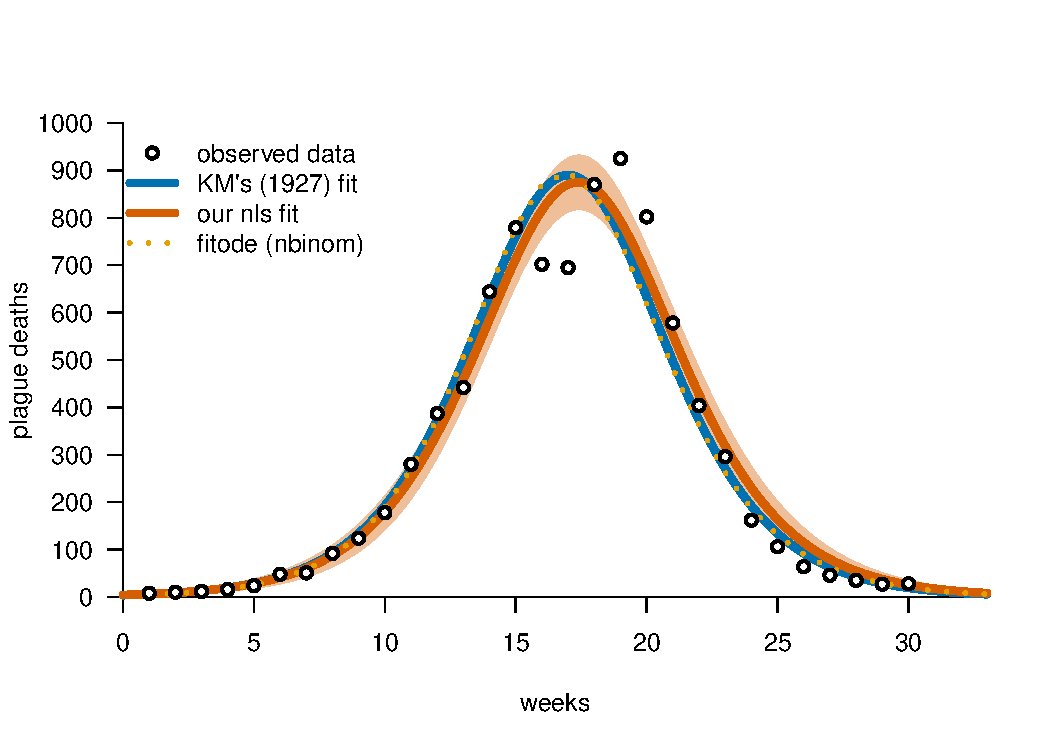
\includegraphics[width=0.95\linewidth]{Bombay-figure-1} 
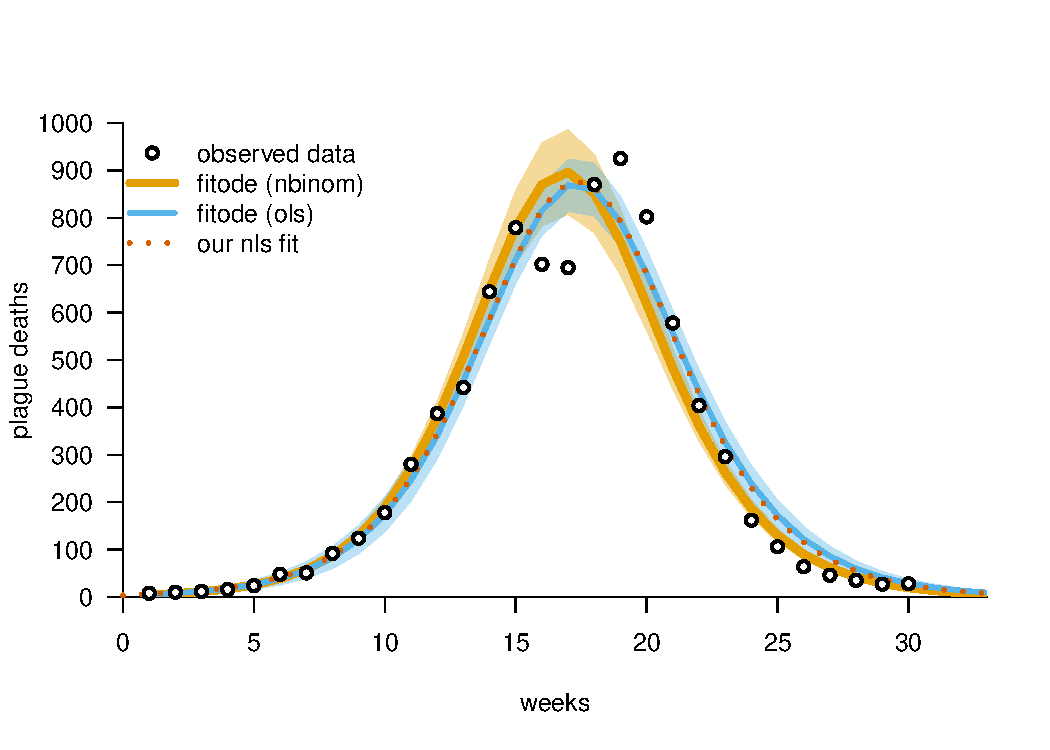
\includegraphics[width=0.95\linewidth]{Bombay-figure-2} 
\end{knitrout}
\caption{\textbf{The plague epidemic in Bombay}, 17 December 1905 to 21 July
  1906, used as an example by \KMpage{714}.  The data
  (large dots) were digitized from \citet[Table~IX, p.\,753]{jhyg1907}.
  \emph{Top panel:} The \KM
  approximation \eqref{eq:sech}, as fitted by \KM (\KMcol curve) and by us
  using \code{nls} (\nlscol curve, with confidence band estimated using the
  Delta method; see \cref{sec:Uncertainty}).  The associated parameter
  estimates are given in \cref{tab:Bombay}.  The dotted \FOnbcol curve
  shows the \code{fitode} fit of the SIR model \eqref{eq:SIR}, for
  which the associated parameter estimates are given in
  \cref{tab:bombay.fitode} [observation errors are assumed to be
    negative binomially distributed \eqref{eq:NB}]; this curve happens to
  coincide almost exactly with KM's fit.
  %%
  \emph{Bottom panel:} The solid \FOnbcol curve is identical to the
  dotted \FOnbcol curve in the top panel; its confidence band is the
  \code{fitode} confidence band obtained by the Delta method [the band
    is shown as a linear interpolation between successive observation
    times because the model \eqref{eq:SIR} is fitted to incidence at
    discrete time points rather than to a continuous curve
    representation of the instantaneous death rate].  The
  \FOolscol curve shows the \code{fitode} fit obtained by
  minimizing the ordinary least squares \eqref{eq:leastsquares} [\ie
    assuming observation errors are normally
    \eqref{eq:prob.data.given.model} distributed with variance
    $\sigma^2$ estimated from the residuals across all observation
    times].  The dotted \nlscol curve is identical to the solid \nlscol curve
  in the top panel.  We have separated the two panels because the
  confidence band overlap would make the plots difficult to
  interpret.}
\label{fig:Bombay}
\end{figure}

%%\begin{landscape}
\begin{table}
  \begin{center}
    \caption{\textbf{Fits of \KM's analytical SIR
        approximation \eqref{eq:sech} to Philadelphia flu} (see
      \cref{fig:phila}).  Parameter estimates were obtained using
      nonlinear least squares (\code{nls}) to fit \cref{eq:sech} to
      the reported daily pneumonia and influenza (P\&I) mortality
      during the main wave of the pandemic in 1918.  In order to
      derive estimates of the standard epidemiological parameters, we
      assumed the initial prevalence had the value estimated by
      \code{fitode} for the SIR model (see \cref{tab:phila.fitode}).
      %%
      We do not use the raw population size in our estimate of $\Rn$;
      instead, we account for the fact that reported deaths are
      roughly equal to incidence times the case fatality proportion
      (CFP) by taking $N$ to be the size of population that would
      eventually die if everyone in the city were infected, \ie the
      product of the population size of Philadelphia in 1918
      (1,768,825) and an assumed
      CFP of $0.025$ \citep{TaubMore06}.
      %%
      The fitted trajectory and confidence band are shown in
      \cref{fig:phila}.  See \cref{sec:phila}.}
    \label{tab:philanls}
    \medskip
    %% making use of ragged2e and array packages:
    \RaggedRight
    \begin{tabular}{ m{3cm} | c | c | c | c c}
      \bfseries Estimated\break parameter & {\footnotesize\bfseries symbol}
      & {\footnotesize\bfseries equation} & {\footnotesize\bfseries units}
      & {\footnotesize\bfseries \code{nls}} & {\footnotesize\bfseries 95\% CI} \\\hline
      total removal rate at epidemic peak & $a$& \eqref{eq:a} & $\frac{1}{\textrm{years}}$ &
      738 & (715, 761) \\
      outbreak speed & $\omega$ & \eqref{eq:omega} & $\frac{1}{\textrm{years}}$ &
      42 & (40.3, 43.5) \\
      outbreak centre & $\phi$ & \eqref{eq:phi} & -- &
      3.64 & (3.51, 3.79) \\
      \noalign{\vspace{10pt}}
      \bfseries Assumed\break parameter \\\hline
      initial prevalence & $\Iinit$ & -- & -- &
      3.05 & -- \\
      effective population size & $N$ & -- & -- &
      44,221 & -- \\
      \noalign{\vspace{10pt}}
      \bfseries Derived\break parameter \\\hline
      peak time & $\tpeak$ & \eqref{eq:tpeak} & weeks &
      4.524 & (4.49, 4.56) \\
      effective reproduction number & $\Reff$
      & \eqref{eq:Reffdef}, \eqref{eq:Reff} & -- &
      128 & (90.8, 165) \\
      \emph{per capita} removal rate & $\gamma$ & \eqref{eq:gamma} & $\frac{1}{\textrm{years}}$ &
      0.66 & (0.492, 0.831) \\
      initial\break susceptibles & $\Sinit$ & \eqref{eq:S0} & -- &
      2270 & (1660, 2880) \\
      transmission rate & $\beta$ & \eqref{eq:beta} & $\frac{1}{\textrm{years}}$ &
      0.0372 & (0.0285, 0.0459) \\
      mean generation interval & $\Tg$ & \eqref{eq:Tg} & years &
      1.52 & (1.12, 1.9) \\
      basic reproduction number & $\Rn$ & \eqref{eq:R0def} & -- &
      2490 & (2416, 2571)
    \end{tabular}
  \end{center}
\end{table}
%%\end{landscape}

%%\begin{landscape}
\begin{table}
  \begin{center}
    \caption{\textbf{Fits of numerical SIR model solutions to Philadelphia flu}
      (see \cref{fig:phila}).
      Parameter estimates are based on \code{fitode} fits of the SIR
      model \eqref{eq:SIR} to reported P\&I mortality during the main
      wave of the 1918 influenza pandemic in the city of Philadelphia.
      As in \cref{tab:philanls}, in order to derive an estimate of
      $\Rn$, we assume an effective population size that accounts for
      the data representing deaths rather than cases.
    }\label{tab:phila.fitode}
    \medskip
    %% making use of ragged2e and array packages:
    \RaggedRight
    \begin{tabular}{ m{3cm} | c | c | c c}
      \bfseries Estimated\break parameter & {\footnotesize\bfseries symbol}
      & {\footnotesize\bfseries units}
      & {\footnotesize\bfseries \code{nbinom}} & {\footnotesize\bfseries 95\% CI} \\\hline
      transmission rate & $\beta$ & $\frac{1}{\textrm{years}}$ &
      0.0124 & (0.0119, 0.0128) \\
      recovery rate & $\gamma$ & $\frac{1}{\textrm{years}}$ & 85.6 &
      (75.9, 96.5) \\
      initial\break susceptibles & $\Sinit$& -- &
      15300 & (14500, 16200)\\
      initial prevalence & $\Iinit$ & -- &
      3.05 & (2.32, 4.01)\\
      overdispersion\break parameter & $k$ & -- &
      157 & (44.2, 557)\\
      \noalign{\vspace{10pt}}
      \bfseries Assumed\break parameter \\\hline
      effective population size & $N$ & -- &
      44,221 &  -- \\
      \noalign{\vspace{10pt}}
      \bfseries Derived\break parameter \\\hline
      effective reproduction number & $\Reff$ & -- &
      2.21 &  (2.02, 2.4) \\
      mean generation interval & $\Tg$ & days &
      4.27 & (3.75, 4.78) \\
      basic reproduction number & $\Rn$ & -- &
      6.38
      &  (5.53, 7.24)
    \end{tabular}
  \end{center}
\end{table}
%%\end{landscape}


\begin{figure}
\begin{knitrout}
\definecolor{shadecolor}{rgb}{0.969, 0.969, 0.969}\color{fgcolor}
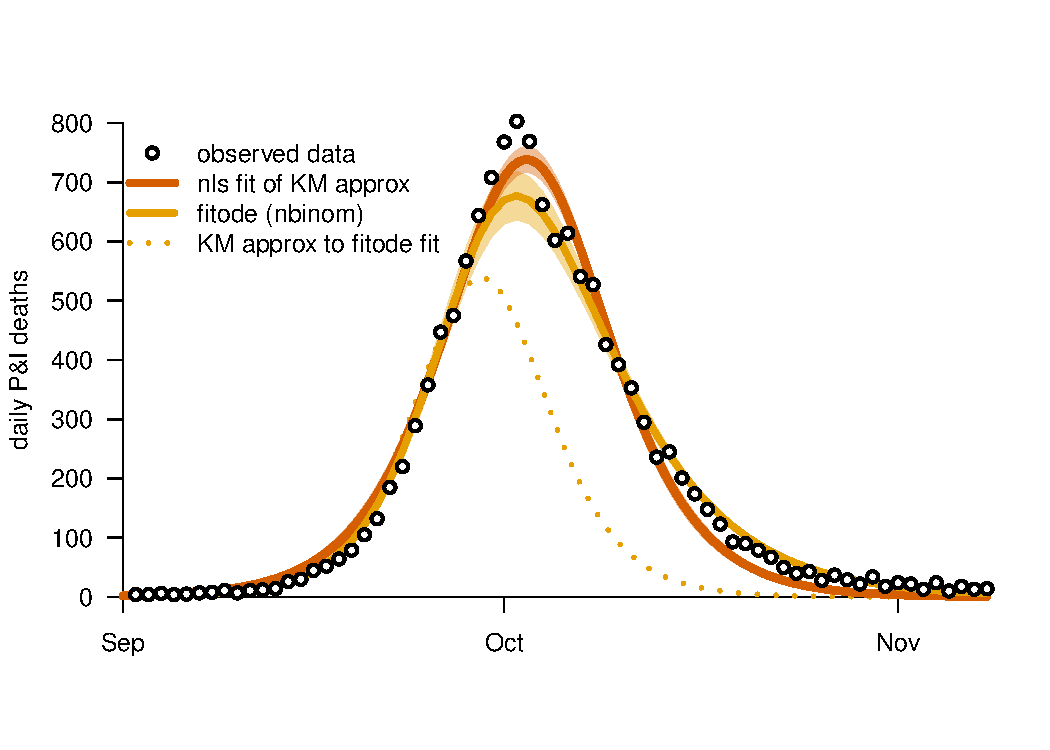
\includegraphics[width=\maxwidth]{phila-figure-1} 
\end{knitrout}
  \caption{\textbf{The main wave of the 1918 influenza epidemic in the city of
      Philadelphia}, 1 September 1918 to 31 December 1918
    \citep{Roge20,Gold+09}.  Reported daily deaths from pneumonia and
    influenza (P\&I) are shown with large dots.  The \nlscol curve and corresponding
    confidence band show a nonlinear least squares (\code{nls}) fit of
    \KM's approximation \eqref{eq:sech}; the parameter estimates are
    given in \cref{tab:philanls}.  The solid \FOnbcol curve and corresponding
    confidence band show the \code{fitode} fit of the SIR model
    \eqref{eq:SIR}, for which the parameter estimates are given in
    \cref{tab:phila.fitode}.  The dotted \FOnbcol curve shows the \KM
    approximation using the parameters estimated with \code{fitode}.
  }
  \label{fig:phila}
\end{figure}

%%\begin{landscape}
\begin{table}
  \begin{center}
    \caption{\textbf{Fits of \KM's analytical SIR
        approximation \eqref{eq:sech} to an epidemic simulated using the
        standard stochastic SIR model \citep{AndeBrit00b}} (see
      \cref{sec:stoch,fig:stoch}).
      %%
      The parameter values in the ``true'' column are those used to
      generate the stochastic simulation ($\Sinit$, $\Iinit$, $\Rn$ and
      $\Tg$) and the values of other parameters derived from these
      true parameter values using the indicated equations.  The
      \code{nls} column lists our estimates and confidence intervals
      obtained by fitting \cref{eq:sech} to the simulated data using
      nonlinear least squares and the Delta method.
    }\label{tab:stoch.nls}
    \medskip
    %% making use of ragged2e and array packages:
    \RaggedRight
    \begin{tabular}{ m{3cm} | c | c | c | c | c c}
      \bfseries Assumed\break parameter & {\footnotesize\bfseries symbol}
      & {\footnotesize\bfseries equation} & {\footnotesize\bfseries units} & {\footnotesize\bfseries true}
      & {\footnotesize\bfseries \code{nls}} & {\footnotesize\bfseries 95\% CI} \\\hline
      initial prevalence & $\Iinit$ & -- & -- &
      2 & 2 & -- \\
      %%
      \noalign{\vspace{10pt}}
      \bfseries Estimated\break parameter \\\hline
      total removal rate at epidemic peak & $a$& \eqref{eq:a} & $\frac{1}{\textrm{weeks}}$ & 641 &
      135 & (125, 144) \\
      outbreak speed & $\omega$ & \eqref{eq:omega} & $\frac{1}{\textrm{weeks}}$ &
      2 & 0.99 & (0.907, 1.08) \\
      outbreak centre & $\phi$ & \eqref{eq:phi} & -- & 3.58 &
      2.7 & (2.48, 2.93) \\
      \noalign{\vspace{10pt}}
      \bfseries Derived\break parameter \\\hline
      peak time & $\tpeak$ & \eqref{eq:tpeak} & weeks &
      1.79 & 2.72 & (2.66, 2.78) \\
      effective reproduction number & $\Reff$
      & \eqref{eq:Reffdef}, \eqref{eq:Reff} & -- &
      5 & 2.62 & (1.79, 3.44) \\
      \emph{per capita} removal rate & $\gamma$ & \eqref{eq:gamma} & $\frac{1}{\textrm{weeks}}$ &
      1 & 1.21 & (0.7, 1.77) \\
      initial\break susceptibles & $\Sinit$ & \eqref{eq:S0} & -- &
      2000 & 571 & (518, 624) \\
      transmission rate & $\beta$ & \eqref{eq:beta} & $\frac{1}{\textrm{years}}$ &
      0.13 & 0.289 & (0.233, 0.346) \\
      mean generation interval & $\Tg$ & \eqref{eq:Tg} & days &
      7 & 5.77 & (3.2, 8.12) \\
      basic reproduction number & $\Rn$ & \eqref{eq:R0def} & -- &
      5
      & 9.18 & (6.95, 11.4)
    \end{tabular}
  \end{center}
\end{table}
%%\end{landscape}

%%\begin{landscape}
\begin{table}
  \begin{center}
    \caption{\textbf{Fits of numerical (deterministic) SIR model solutions to
        an epidemic simulated using the standard stochastic SIR model
        \citep{AndeBrit00b}} (see \cref{sec:stoch,fig:stoch}). Parameter
      estimates we obtained using \code{fitode} to fit the SIR model
      \eqref{eq:SIR} to the simulated data, assuming deviations from
      the deterministic curve were generated by negative binomially
      \eqref{eq:NB} distributed observation errors.
    }\label{tab:stoch.fitode}
    \medskip
    %% making use of ragged2e and array packages:
    \RaggedRight
    \begin{tabular}{ m{3cm} | c | c | c | c c}
      \bfseries Estimated\break parameter & {\footnotesize\bfseries symbol}
      & {\footnotesize\bfseries units} & {\footnotesize\bfseries true}
      & {\footnotesize\bfseries \code{nbinom}} & {\footnotesize\bfseries 95\% CI} \\\hline
      transmission rate & $\beta$ & $\frac{1}{\textrm{years}}$ & 0.13 &
      0.131 & (0.119, 0.144) \\
      recovery rate & $\gamma$ & $\frac{1}{\textrm{weeks}}$ & 1 &
      0.971 & (0.884, 1.07)\\
      initial\break susceptibles & $\Sinit$& -- & 1998 &
      2000 & (1900, 2110)\\
      initial prevalence & $\Iinit$ & -- & 2 &
      0.605 & (0.306, 1.2)\\
      overdispersion\break parameter & $k$ & -- & -- &
      251 & (  19.6, 3226.6)\\
      \noalign{\vspace{10pt}}
      \bfseries Derived\break parameter \\\hline
      mean generation interval & $\Tg$ & days & 7 & 7.21 & (7.92, 6.56)\\
      effective reproduction number & $\Reff$ & -- & 4.995 &
      5.2 &  (4.44, 5.95) \\
      basic reproduction number & $\Rn$ & -- & 5 &
      5.19
      &  (4.37, 6.01)
    \end{tabular}
  \end{center}
\end{table}
%%\end{landscape}

\begin{figure}
\begin{knitrout}
\definecolor{shadecolor}{rgb}{0.969, 0.969, 0.969}\color{fgcolor}
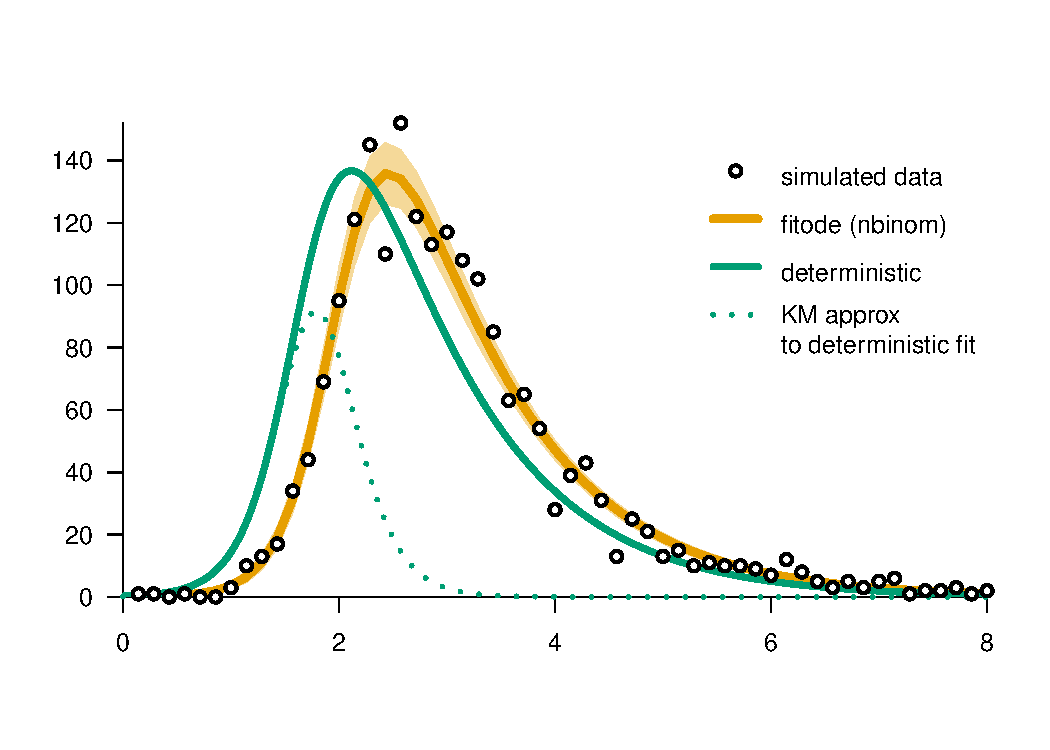
\includegraphics[width=0.95\linewidth]{plot_stochastic_SIR-1} 
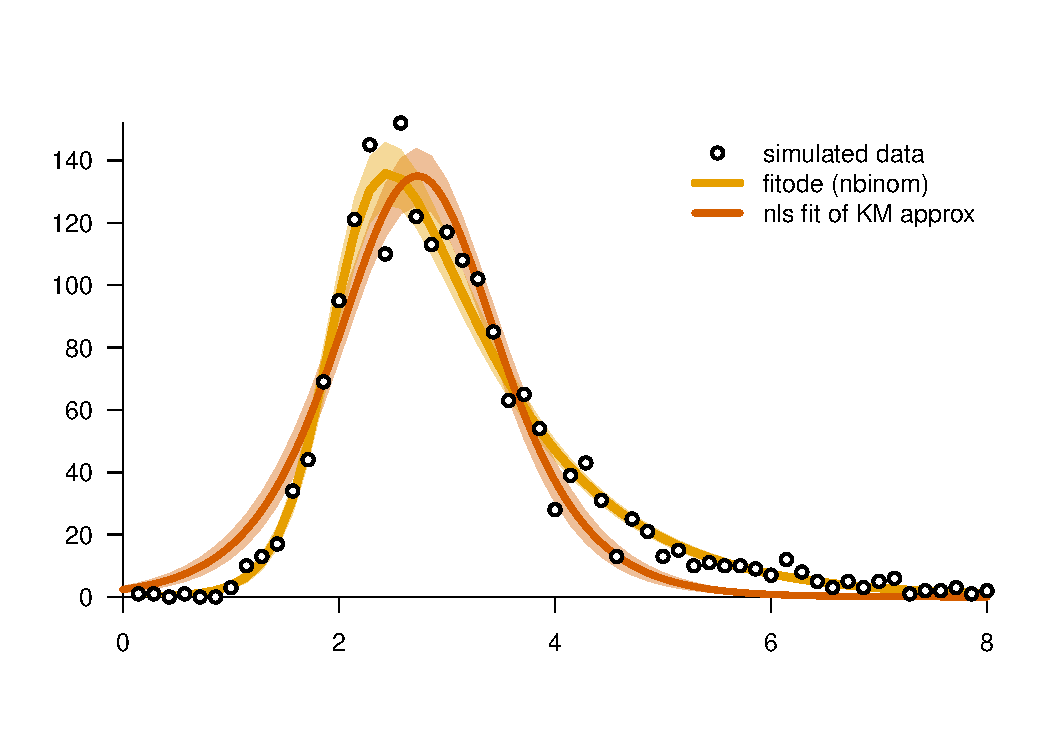
\includegraphics[width=0.95\linewidth]{plot_stochastic_SIR-2} 
\end{knitrout}
  \caption{\textbf{Deterministic fits to daily incidence generated by a
      stochastic SIR simulation} with initial state
    $(\Sinit,\Iinit,\Rinit)=(1998,2,0)$, basic reproduction number $\Rn=5$, and
    mean generation interval $\Tg=1$ week.
    The simulated data points show the numbers of newly recovered
    individuals each day.
    %%
    In both panels, the \FOnbcol curve and confidence band show the
    \code{fitode} fit to the simulated data.  \emph{Top panel:} The
    solid \determcol curve shows the solution of deterministic SIR model
    \eqref{eq:SIR} with the initial conditions and parameters used for
    the stochastic simulation.  The dotted \determcol curve shows the \KM
    approximation \eqref{eq:sech} to this deterministic trajectory.  The
    time shift between the \determcol and \FOnbcol curves arises because there
    is a random delay until the stochastic trajectory begins to grow
    exponentially.
    %%
    \emph{Bottom panel:} The \nlscol curve shows the \KM approximation
    \eqref{eq:sech}, fitted to the stochastic simulation using \code{nls}.
    Since the \KM approximation is symmetric about its maximum, it is
    impossible to obtain a good fit in situations like this, where
    the rise of the epidemic is faster than the fall.
  }\label{fig:stoch}
\end{figure}

\pagebreak

\begin{figure}[!h]
  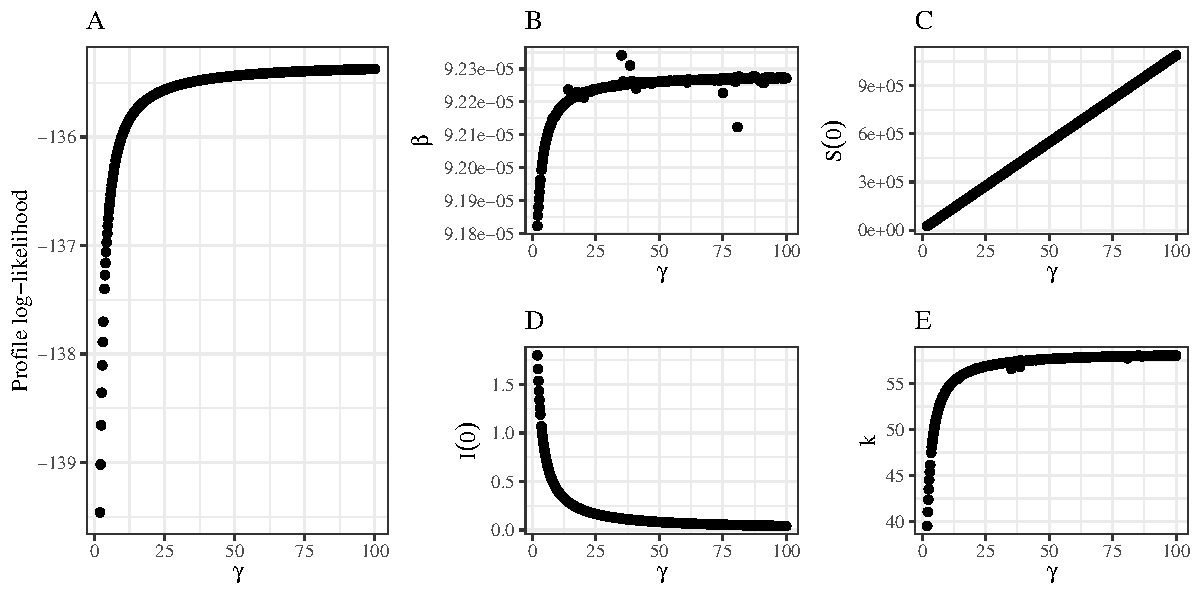
\includegraphics[width=\textwidth]{bombay_confint_dnbinom.pdf}
  \caption{\textbf{Unidentifiability of the mean generation interval
      $\Tg$ (or, equivalently, the \emph{per capita} removal rate $\gamma$) for the Bombay
      plague epidemic shown in \cref{fig:Bombay}.}
    %%
    (\textsf{A}) The profile likelihood---briefly discussed at the end
    of \cref{sec:Uncertainty}---is calculated by fixing $\gamma$ to a
    series of given values and, for each value,
    maximizing the likelihood by estimating all other
    parameters \citep{Bolk08}. (The maximum value is shifted to 0
    without loss of generality.) A flat profile-likelihood surface
    indicates parameter unidentifiability, meaning that we can obtain
    very similar fits across a wide range of values
    of the focal parameter ($\gamma$).  (\textsf{B--E}) The
    corresponding best parameter estimates for a given value of
    $\gamma$.}\label{fig:proflikgamma}
\end{figure}

\end{document}
